% TODO:
% - Go through quoting in the text, for example: so-called "", '' or just \emph{text} or \textit{text} === MUST BE CONSISTENT
% - Go through numbering in the text, use either words: one, two, or numbers: 1, 2

\chapter{Theory \TO}
This chapter will present the core theory of areas used in this research assignment. Firstly, Graphical Processing Units (GPUs) will be introduced with an emphasis on the architecture of GPUs (only Nvidia GPUs as the Nvidia API, CUDA, was used to develop this project). Then, CUDA, will be described in greater detail. Finally, the theory behind Lower-Upper (LU) Decomposition will be presented.

\section{GPUs \TO}
From an average consumer's perspective a Graphics Processing Unit (GPU) is a component of a computing system that performs graphical operations, for example, processing images. For the sake of the example, let image processing be simplified into the following: images are composed of pixels and each pixel needs to be processed. Since a GPU contains thousands of processing units it can perform a large number of operations in parallel, for example, processing a large number of pixels at once, thus making it highly efficient at image processing. While this has a wide range of uses, there is another field where the highly-parallel nature of the GPU can be utilized: General-Purpose Computing on Graphics Processing Units (GPGPU).

\subsection{General-Purpose Computing on Graphics Processing Units (GPGPU) \TO}
As described in section 1.2 of the author's bachelor thesis \textit{Formats for storage of sparse matrices on GPU} \cite{Cejka2020}, GPUs started to evolve at the turn of the 21st century from purely graphics-processing units into devices capable of general-purpose computing, i.e. computation that is not necessarily related to graphics. The significance of this event lies in the use of graphics cards for seemingly any parallelizable computational task that would benefit from the abundance of slower processing units on a GPU rather than fewer faster processing units found on a CPU \cite{NVIDIAMay2022}.

\par For reference, high-end desktop CPUs today usually have anywhere from 8 to 16 cores, while server CPUs can have upwards of 64 cores (not counting hyper-threading and similar technologies). In general, CPUs with more cores have a lower clock speed - see figure~\ref{Figure:processor-comparison} for a selection of processors along with their core count and clock speeds \cite{Glawion7March2022}.

\begin{figure}[H]
	\centering
	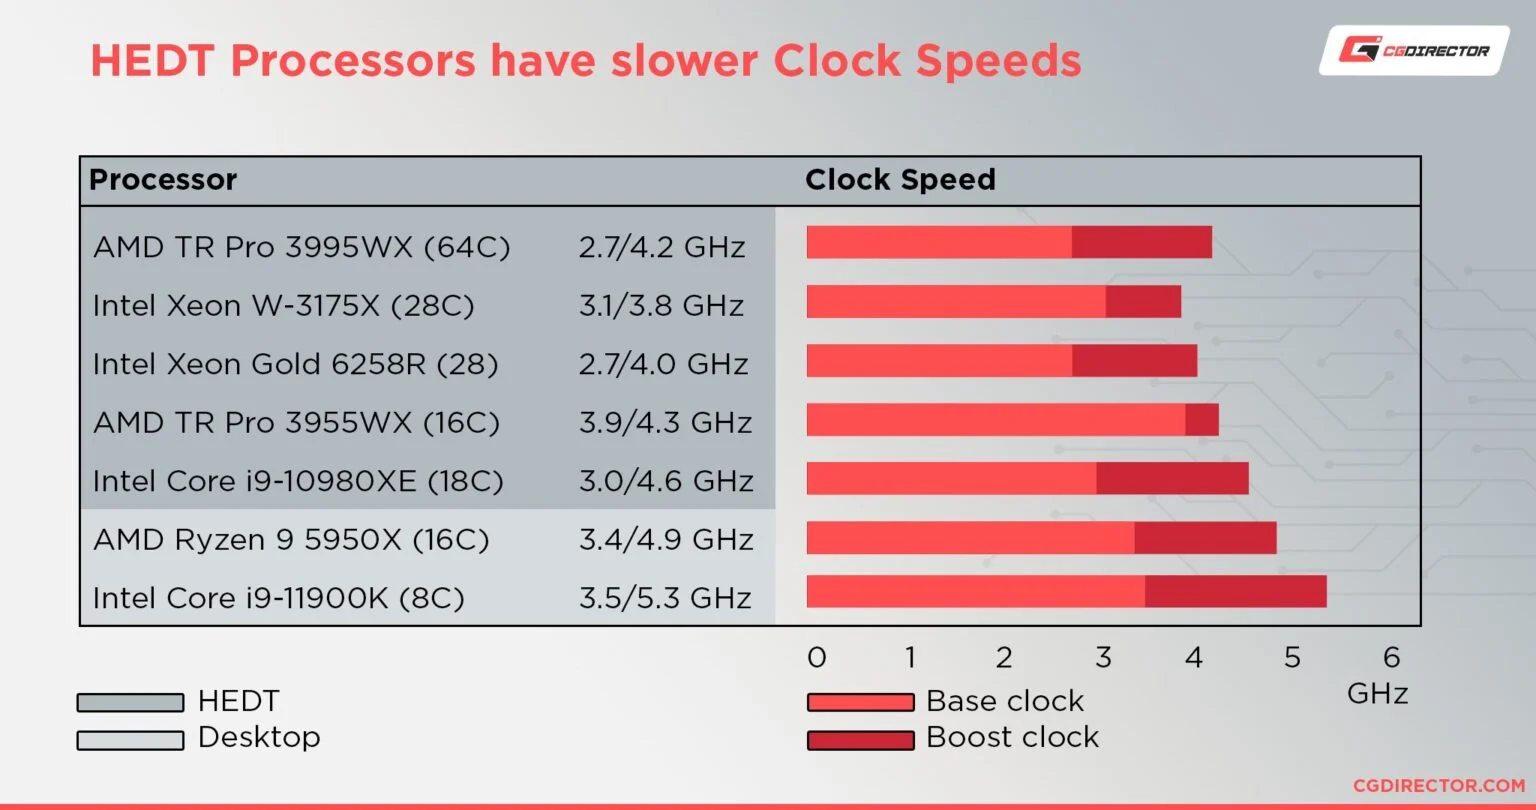
\includegraphics[width=14cm, keepaspectratio]{images/ch1/processors_comparison.png}
	\caption{Selection of desktop and server CPUs - including number of cores and clock speed \cite{Glawion7March2022}. HEDT stands for High-End Desktop Processor - in this instance it also includes CPUs predominantly used in servers.}
	\label{Figure:processor-comparison}
\end{figure}

While CPUs are widely used for sequential tasks, they can also be used for tasks that can be described as parallelizable, for example, processing of requests to a server. They are not suitable for highly parallel tasks such as image processing, where GPUs excel due to their architecture. Figure~\ref{Figure:Nvidia-CPU-GPU-architecture-comparison} shows the comparison of a CPU and GPU architecture. The example CPU in the figure has - among other components - 4 cores each having its own L1 cache and controlling component. This configuration allows for executing a thread (series of operations) at a high speed and lower throughput (fewer number of threads running at once). Simply, the CPU is more suitable for rapid completion of serialized instructions.

\begin{figure}[h!]
	\centering
	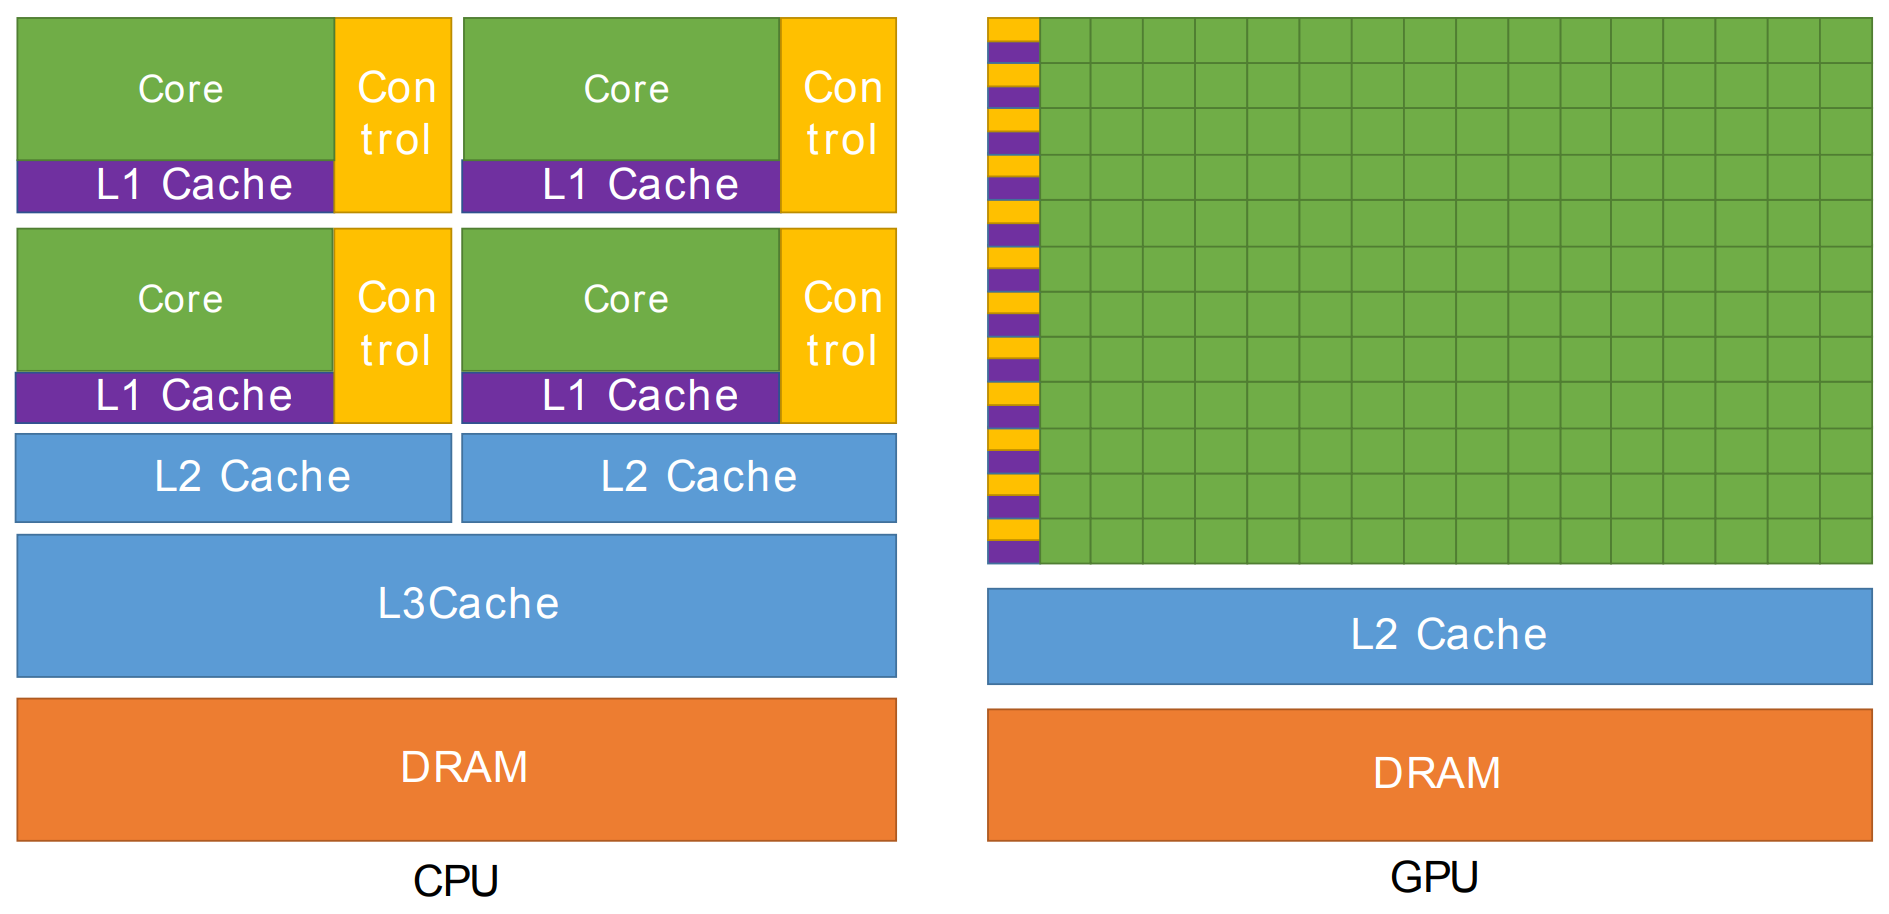
\includegraphics[width=14cm, keepaspectratio]{images/ch1/nvidia_CPU_GPU_comparison.png}
	\caption{Comparison of the architecture of CPUs and GPUs. On one hand, CPUs have fewer cores, more complex controlling logic compared to GPUs and the cores of a CPU have a higher clock speed. On the other hand, GPUs have a much higher number of cores clocked at lower speeds. Taken from Nvidia's \emph{CUDA C++ programming guide} \cite{NVIDIAMay2022}.}
	\label{Figure:Nvidia-CPU-GPU-architecture-comparison}
\end{figure}

Nvidia GPUs, on the other hand, are engineered to have many smaller controlling units called SMs (Stream Multiprocessors) that aim to schedule and task individual processing units found on the GPU. Furthermore, in figure~\ref{Figure:Nvidia-CPU-GPU-architecture-comparison} it can be seen that GPUs have a different cache structure. Specifically, GPUs only have two levels, whereas CPUs have three. In summary, the GPU has more transistors for processing data - namely operations that use floating-point computations. Moreover, the architecture of the GPU allows for it to compensate for memory access delays by performing computations simultaneously \cite{NVIDIAMay2022}.
\par A prime example of where this characteristic gives a significant advantage to the GPU over the CPU is during matrix multiplication which will be described later in subsection~\ref{Subsection:matrix-multiplication}.

\par For completion, see table~\ref{Table:Nvidia-gpu-details-comparison} for a selection of GPUs along with their specifications.

\begin{table}[h!]
	\centering
	\renewcommand{\arraystretch}{0.9}
	\begin{tabular}{|>{\raggedright\arraybackslash\bfseries\scriptsize}m{2.7cm}|>{\scriptsize}m{2.7cm}|>{\scriptsize}m{2.7cm}|>{\scriptsize}m{2.7cm}|>{\scriptsize}m{2.7cm}|}
		\hline
		\rowcolor{nvidia}\multicolumn{1}{|>{\centering\arraybackslash\normalsize}m{2.72cm}|}{$\vcenter{\textbf{Nvidia}}$} 
		& \multicolumn{1}{>{\centering\arraybackslash\normalsize}m{2.72cm}|}{$\vcenter{\textbf{GTX 1070}}$}
		& \multicolumn{1}{>{\centering\arraybackslash\normalsize}m{2.72cm}|}{$\vcenter{\textbf{RTX 3060}}$}
		& \multicolumn{1}{>{\centering\arraybackslash\normalsize}m{2.72cm}|}{$\vcenter{\textbf{V100}}$}
		& \multicolumn{1}{>{\centering\arraybackslash\normalsize}m{2.72cm}|}{$\vcenter{\textbf{A100}}$}\\[5pt]
		\hline
		GPU & GP104 (Pascal) & GA106 (Ampere) & GV100 (Volta) & GA100 (Ampere) \\
		\hline
		\rowcolor{lightnvidia}\multicolumn{1}{|>{\arraybackslash\bfseries\scriptsize}m{2.72cm}|}{SMs}
		& \multicolumn{1}{>{\arraybackslash\scriptsize}m{2.72cm}|}{15}
		& \multicolumn{1}{>{\arraybackslash\scriptsize}m{2.72cm}|}{28}
		& \multicolumn{1}{>{\arraybackslash\scriptsize}m{2.72cm}|}{80}
		& \multicolumn{1}{>{\arraybackslash\scriptsize}m{2.72cm}|}{108} \\
		\hline
		TPCs & 15 & 14 & 40 & 54 \\
		\hline
		FP32 Cores / SM & NA &NA & 64 & 64 \\
		\hline
		FP32 Cores / GPU & NA & NA & 5120 & 6912 \\
		\hline
		FP64 Cores / SM & NA & NA & 32 & \\
		\hline
		FP64 Cores / GPU (excl. Tensor)	& NA & NA & 2560 & 3456 \\
		\hline
		CUDA Cores / SM & 128 & 128 & NA & NA \\
		\hline
		CUDA Cores / GPU & 1920 & 3584 & NA & NA \\
		\hline
		Tensor Cores / SM & NA & 4 & 8 & 16 \\
		\hline
		Tensor Cores / GPU & NA & 112 & 640 & 432 \\
		\hline
		GPU Boost Clock & 1683 MHz & 1777 MHz & 1530 MHz & 1410 MHz \\
		\hline
		\rowcolor{lightnvidia}\multicolumn{1}{|>{\arraybackslash\bfseries\scriptsize}m{2.72cm}|}{Peak FP32 TFLOPS}
		& \multicolumn{1}{>{\arraybackslash\scriptsize}m{2.72cm}|}{6.5}
		& \multicolumn{1}{>{\arraybackslash\scriptsize}m{2.72cm}|}{12.7}
		& \multicolumn{1}{>{\arraybackslash\scriptsize}m{2.72cm}|}{15.7}
		& \multicolumn{1}{>{\arraybackslash\scriptsize}m{2.72cm}|}{19.5}\\
		\hline
		\rowcolor{lightnvidia}\multicolumn{1}{|>{\arraybackslash\bfseries\scriptsize}m{2.72cm}|}{Peak FP64 TFLOPS}
		& \multicolumn{1}{>{\arraybackslash\scriptsize}m{2.72cm}|}{0.202}
		& \multicolumn{1}{>{\arraybackslash\scriptsize}m{2.72cm}|}{0.199}
		& \multicolumn{1}{>{\arraybackslash\scriptsize}m{2.72cm}|}{7.8}
		& \multicolumn{1}{>{\arraybackslash\scriptsize}m{2.72cm}|}{9.7}\\
		\hline
		Peak Tensor TFLOPS & NA & 51 & 125 & 312/624$^3$\\
		\hline
		\rowcolor{lightnvidia}\multicolumn{1}{|>{\arraybackslash\bfseries\scriptsize}m{2.72cm}|}{Memory Bandwidth}
		& \multicolumn{1}{>{\arraybackslash\scriptsize}m{2.72cm}|}{256 GB/s}
		& \multicolumn{1}{>{\arraybackslash\scriptsize}m{2.72cm}|}{360 GB/s}
		& \multicolumn{1}{>{\arraybackslash\scriptsize}m{2.72cm}|}{900 GB/s}
		& \multicolumn{1}{>{\arraybackslash\scriptsize}m{2.72cm}|}{1555 GB/s} \\
		\hline
		Texture Units & 120 & 112 & 320 & 432 \\
		\hline
		Memory Interface & 256-bit & 192-bit & 4096-bit HBM2 & 5120-bit HBM2 \\
		\hline
		Memory Size & 8 GB & 12 GB & 32 GB & 80 GB \\
		\hline
		L2 Cache Size & 2048 KB & 3072 KB & 6144 KB & 40960 KB \\
		\hline
		Shared Memory Size / SM & 96 KB & 128 KB & Configurable up to 96 KB & Configurable up to 164 KB \\
		\hline
		Register File Size / SM & 256 KB & 256 KB & 256 KB & 256 KB \\
		\hline
		Register File Size / GPU & 3840 KB & 7168 KB & 20480 KB & 27648 KB \\
		\hline
		\rowcolor{lightnvidia}\multicolumn{1}{|>{\arraybackslash\bfseries\scriptsize}m{2.72cm}|}{TDP}
		& \multicolumn{1}{>{\arraybackslash\scriptsize}m{2.72cm}|}{150 Watts}
		& \multicolumn{1}{>{\arraybackslash\scriptsize}m{2.72cm}|}{170 Watts}
		& \multicolumn{1}{>{\arraybackslash\scriptsize}m{2.72cm}|}{300 Watts}
		& \multicolumn{1}{>{\arraybackslash\scriptsize}m{2.72cm}|}{400 Watts}\\
		\hline
		Transistors & 7.1 billion & 12 billion & 21.1 billion & 54.2 billion \\
		\hline
		GPU Die Size & 314 mm$^2$ & 276 mm$^2$ & 815 mm$^2$ & 826 mm$^2$\\
		\hline
		Manufacturing Process & TSMC 16nm & Samsung 8N & 12 nm FFN & 7 nm N7\\
		\hline
	\end{tabular}
	\caption{Comparison of GPUs: GTX 1070 (Turing architecture), RTX 3060 (Ampere architecture), V100 (Volta architecture), A100 (Ampere architecture). The GPUs in this table assume the best possible configuration of their respective card, for example, the version with the most possible VRAM. Features that are important when it comes to card performance have been denoted in green. The data was obtained from various sources for the GTX 1070 \cite{Hagedoorn6October2016, oaUUFoT7oI5ApIyY, Smith18May2016, jAnwkq6mMKYTLUOB} the RTX 3060 \cite{Walton7July2021, wGXr33zSUweXiQMY, SMhyh0H3oh3nlda0, May1December2020} and the A100 \cite{soj8qSRbfefUdi8Y, rfiOEXAGDlcAOxF3}.}
	\label{Table:Nvidia-gpu-details-comparison}
\end{table}

The table shows specifications for two different categories of GPUs: consumer and professional (commercial). Consumer cards (in the table: GTX 1070, RTX 3060) can be found in regular desktop PCs and are intended more for video gaming, rather than raw computing power. However, these cards are mentioned as the optimization of this project's implementation was done on machines that included them. On the other hand, professional cards are intended mainly for GPGPU, or - in some specific cases - for machine learning. \\
Characteristics that can be used to compare GPUs are, for example, peak TFLOPS (TFLOPS - how many trillion floating-point operations can the processor perform per second), memory bandwidth, TDP. The value that clearly separates commercial cards from consumer cards is the peak FP64 (double precision) TFLOPS, which is the highest for the A100 at 9.7 TFLOPS, with the V100 being slightly slower at 7.8 TFLOPS, whereas the consumer cards perform significantly worse at around 0.2 TFLOPS. \\
In summary, professional cards are heavily preferred when it comes to GPGPU, however, consumer cards can be and are used for development as they are more affordable.



\section{Compute Unified Device Architecture (CUDA) \TO}\label{Section:CUDA}
The Compute Unified Device Architecture (CUDA) is programming model, sometimes referred to as a parallel computing platform, introduced by Nvidia in 2006 \cite{Oh10September2012}. It is designed to give developers low-level access to GPU hardware, for example, fine-tuning assignment of processing units or memory allocation, thus, allowing them to utilize the full potential of GPUs and tailor their use for specific applications. CUDA supports a variety of programming languages, for example, C++ (used in this project) and Fortran, however, adaptations for other languages such as, Python, Perl, Java, Ruby, MATLAB, Julia, etc. have been created \cite{OsGyRFLMngy0j8Pv}.
\par This section will first explain some basic terminology followed by the theory behind CUDA from the simplest concept - a thread - to how threads are managed. Then, memory will be introduced in a similar manner: from per-thread local memory to global memory. Subsequently, asynchronous concurrent execution will be described. Finally, basic CUDA extensions of the C++ language will be presented and their translation into the thread and memory management systems will be shown on a simple example program.

\subsection{Introductory terminology \TO}\label{Subsection:CUDA-introductory-terminology}
CUDA introduces many unique concepts that come with their own naming scheme. This subsection will list and explain some basic terminology that will be used throughout the project \cite{Ruetsch2008}:
\begin{itemize}
	\item \textbf{Host} - Central Processing Unit (CPU) and its memory. The host provides data to GPU and instructs it to execute various instructions.
	\item \textbf{Device} - Graphics Processing Unit (GPU) and its memory. The device executes specialized instructions provided by the host.
	\item \textbf{Kernel} - term used for a special type of function that, unlike regular functions, can only be called from the host and executed on the device. Furthermore, when a CUDA kernel is called it is executed in parallel across a number of threads.	
\end{itemize}

\subsection{Thread Management \TO}\label{Subsection:thread-management}
This subsection will aim to describe how CUDA handles its basic execution units: threads. First, a thread itself will be defined and described followed by explanations of multiple encompassing thread structures.

\paragraph{CUDA thread}
The thread management system within CUDA begins, at the most basic level, with its smallest execution unit, a thread. According to \emph{CUDA C++ Programming Guide} a thread is an executed sequence of operations \cite{NVIDIAMay2022}. Due to the highly-parallel nature of the GPU - spreading the workload across thousands of execution units - a CUDA thread is designed to be lightweight (unlike a typical CPU thread - assuming no hyper-threading is present). In this context, 'lightweight' signifies that the GPU is capable of easily switching between threads. An example showing how a set of instructions can be run on a set of 8 threads can be seen in figure~\ref{Figure:CUDA-thread-parallelism}. \\
In this project, the terms 'CUDA thread' and 'thread' will be used interchangeably. For a more detailed explanation of the difference between a CUDA thread and that of the CPU see \emph{Formats for storage of sparse matrices on GPU} \cite{Cejka2020}.

\begin{figure}[h!]
	\centering
	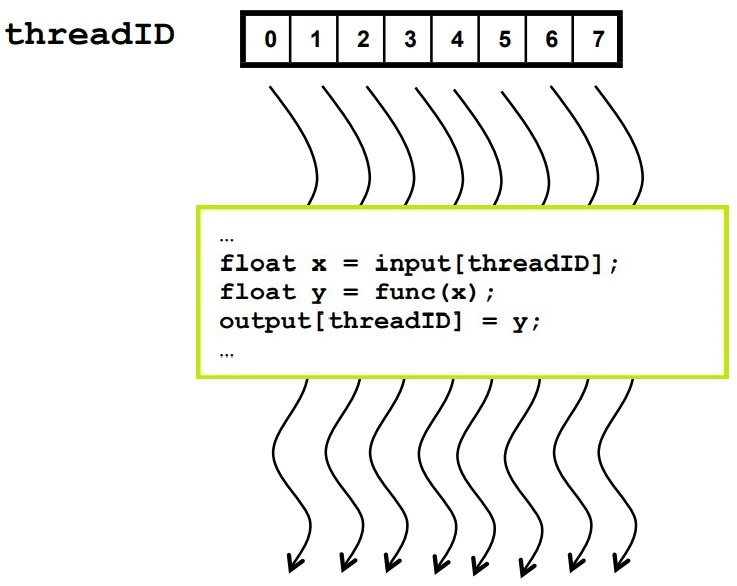
\includegraphics[width=9.5cm, keepaspectratio, clip]{images/ch1/CUDA_thread_parallelism.jpg}
	\caption{On an Nvidia GPU, eight threads with IDs from \code{0} to \code{7} execute the code in this example. A value from the array \code{input} with \code{threadID} as the index (i.e. each thread will read a value at a different index) is changed using the function \code{func(x)} and then stored in the same order as before into the array \code{output}. Taken from \emph{Format for storage of sparse matrices on GPU} \cite{Cejka2020, Ruetsch2008}.}
	\label{Figure:CUDA-thread-parallelism}
\end{figure}

\paragraph{Warp}
To execute thousands of threads simultaneously, SMs of an Nvidia GPU use the Single-Instruction Multiple-Thread (SIMT) execution model. The abbreviation SIMT comes from the amalgamation of SIMD (Single-Instruction Multiple-Data) and multi-threading (executing multiple sequences of instructions simultaneously). Specifically, this approach comprises of multiple threads executing the same computations on different data items \cite{Marziale2010}. In terms of CUDA, the core of the SIMT architecture is a so-called 'warp' that is made up of 32 threads. In other words, the smallest number of threads that can be executed simultaneously is 32. If fewer threads are required, for example, only 1 thread, then CUDA will still allocate 32 threads with 31 being inactive. Similarly, if a subset of threads from a warp are to execute different instructions (e.g., as a result of a conditional statement) then the different sets of instructions are executed serially across their respective threads - this issue is known as 'thread divergence'. An example of thread divergence can be seen in figure~\ref{Figure:CUDA-warp-thread-divergence}; the warp in the example is simplified for the purpose of the explanation and as such contains only 8 threads.

\begin{figure}[h!]
	\centering
	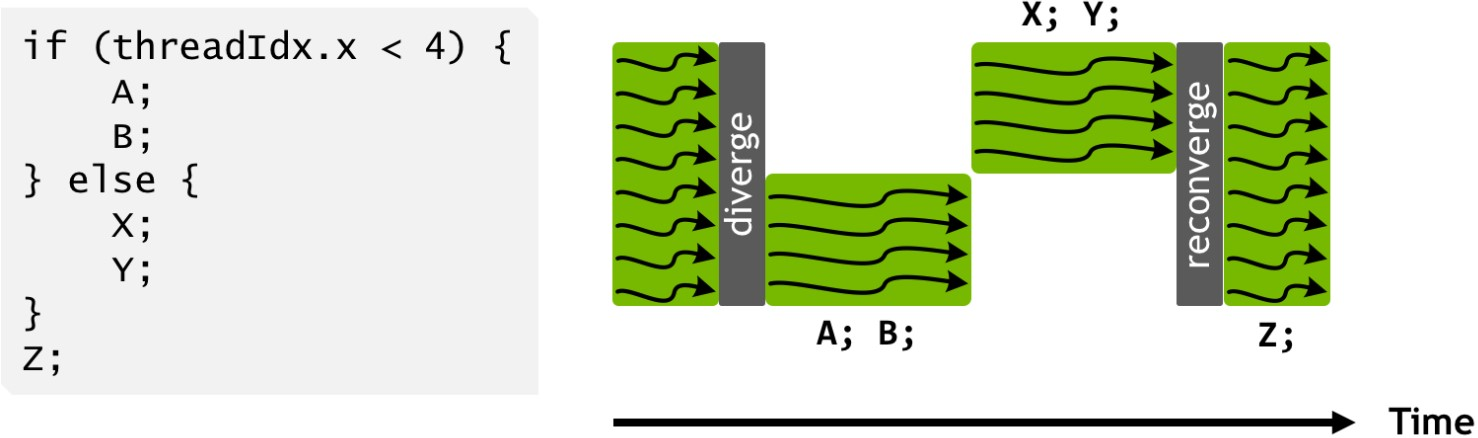
\includegraphics[width=14cm, keepaspectratio]{images/ch1/CUDA_warp_divergence_execution_path.jpg}
	\caption{Conditional code execution by a warp of 8 threads; each thread is represented by one wavy line. Due to the condition, threads with an ID between \code{0} and \code{3} will only execute statements \code{A} and \code{B}. However, simultaneously, threads with IDs between \code{4} and \code{7} will be put on hold. Comparably, while threads with IDs between \code{4} and \code{7} will be executing statements \code{X} and \code{Y}, the remaining threads will be idle. Thus, thread divergence has occurred within the 8-thread warp. Taken from Nvidia's developer blog post: \emph{Inside Volta: The World's Most Advanced Data Center GPU} \cite{Durant10May2017}.}
	\label{Figure:CUDA-warp-thread-divergence}
\end{figure}
\footnotetext{L. Durant, O. Giroux, M. Harris: \emph{Inside Volta: The World’s Most Advanced Data Center GPU}. URL: \protect\url{https://devblogs.nvidia.com/inside-volta/}}

\paragraph{Block}
It is not always necessary to use such granularity that warps are able to provide. Developers can choose to execute code on a group of up to 1024 threads (with CUDA Compute Capability greater than 3.5) - referred to as a block. Threads in a block can cooperate via shared memory (subsection \ref{Subsection:memory-management} will explain more) and they can be synchronized - this is not possible for threads in different blocks. Threads in a block can be structured in 1, 2, or 3 dimensions (x, y, z); each thread has a unique ID in every dimension. The 1024 threads-per-block limit encompasses all 3 possible dimensions, in other words, the total number of threads must be at most 1024 across all dimensions (\code{num\_threads\_x\_dim} $ \cdot $ \code{num\_threads\_y\_dim} $ \cdot $ \code{num\_threads\_z\_dim} $ \leq$ 1024) \cite{AbiChahla18June2008, NVIDIAMay2022}.

\paragraph{Grid}\label{Paragraph:CUDA-thread-management-grid}
In terms of CUDA a grid consists of multiple blocks of threads. Similarly to how threads can be structured within blocks, blocks can be structured within grids - up to 3 dimensions of blocks; each block has a unique ID in every dimension. The maximum number of blocks in every dimension is set to $ 2^{31} - 1 $ (65 536). One of the main reasons for having another structure on top of blocks (apart from memory management - detailed explanation in subsection~\ref{Subsection:memory-management}) stems from the fact that while the limit for threads per block is set to 1024, GPUs are capable of running a multitude more threads in parallel. This means that the grid structure allows for the same code to be executed simultaneously on a group of thread blocks. However, it is important to note that there is a limit of how many threads can be active at once. When this limit is reached, blocks of threads are executed sequentially in such a way that allows for near-maximal concurrently active threads. Another noteworthy aspect is the difference between the terms 'number of allocated threads' and 'number of active threads'. The former means how many threads are allocated in total, i.e. both active (currently executing) and inactive (scheduled) threads, whereas the latter refers to threads that are actively being executed at a point in time. \\
A visualization of CUDA's thread structuring can be seen in figure~\ref{Figure:CUDA-grid-block-thread}.

\begin{figure}[h!]
	\centering
	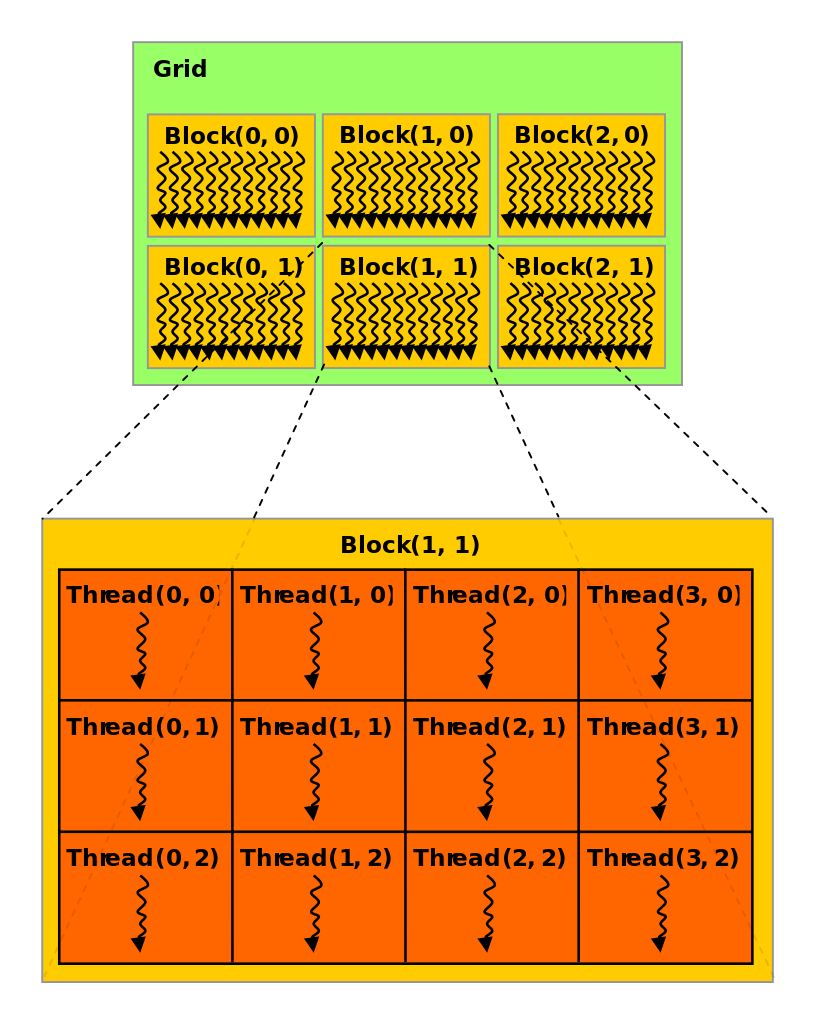
\includegraphics[width=11cm, keepaspectratio]{images/ch1/nvidia_grid_block_thread.png}
	\caption{CUDA thread structuring of a 2D grid made up of 2D blocks of threads. Taken from Nvidia's \emph{CUDA C++ Programming Guide} \cite{NVIDIAMay2022}.}
	\label{Figure:CUDA-grid-block-thread}
\end{figure}


\subsection{Memory Management \TO}\label{Subsection:memory-management}
The aim of this subsection is to present how memory management works in CUDA. Different types of memory available on the GPU will be presented, ranging from per-thread local to global memory.

\paragraph{Per-thread local memory}
When a kernel is executed on the GPU across a number of threads every thread has its own unique ID stored in a variable that is available within the kernel. This variable is stored in memory that is referred to as \textit{per-thread local memory}. In other words, every thread has its own local memory where it can store variables. It is important to note that per-thread local memory consists of two different types - registers and local memory. Registers is on-chip memory (low latency and high bandwidth), however, it is limited in capacity at 255 32-bit registers per thread in CUDA Compute Capability 3.5 and higher, which does not allow for extensive kernels containing many variables. The compiler will store almost all variables allocated within the kernel into registers, with the exception of \cite{NVIDIAMay2022}:
\begin{itemize}
	\item Arrays indexed with constant quantities
	\item Large structures or arrays that would use too much registers space
	\item Any variable if the kernel uses more registers than available - called \textit{register spilling}
\end{itemize}
The variables and structures mentioned above that the compiler will not store in registers will instead be stored in purely local memory which resides in device memory. Device memory is also referred to as global memory which is off-chip and therefore, any accesses by threads into their purely local memory will be slower than accessing registers. Figure~\ref{Figure:CUDA-memory-types-detailed} shows available accesses of threads to different types of memory. \\
As of CUDA Compute Capability 3.5, the amount of purely local memory available for every thread is only 512 KB \cite{NVIDIAMay2022}. In summary, per-thread local memory is often used sparingly to avoid register spilling and the accompanied slower memory access, however, if used efficiently, it can be helpful when complex indexing is required for some calculations.

\paragraph{Shared memory}\label{Paragraph:CUDA-memory-management-shared-memory}
The next layer of memory is per-block memory referred to as \textit{shared memory}. As the name suggests, this memory is shared by all threads belonging to a particular block. Similarly to registers, shared memory is on-chip and therefore it is fast, however, it is also limited in capacity depending on the CUDA Compute Capability version - see table \ref{Table:CUDA-block-max-shared-memory} for specific values.

\begin{table}[h!]
	\centering
	\renewcommand{\arraystretch}{1.5}
	\begin{tabular}{ |c|c|c|c|c|c|c| } 
		\hline
		Compute Capability & 3.5 - 6.2 & 7.0 - 7.2 & 7.5 & 8.0 & 8.6 & 8.7 \\
		\hline
		Max. shared memory per block [KB] & 48 & 96 & 64 & 163 & 99 & 163 \\
		\hline
	\end{tabular}
	\caption{Maximum shared memory per thread block across different CUDA Compute Capabilities. Nvidia notes in their documentation that any value above 48 KB requires the use of dynamic shared memory. Taken from Nvidia's \emph{CUDA C++ Programming Guide} \cite{NVIDIAMay2022}.}
	\label{Table:CUDA-block-max-shared-memory}
\end{table}

Shared memory can either be allocated statically or dynamically. The former needs the size of allotted memory to be known at compile time, for example, an array of constant size denoted within the kernel using a dedicated prefix that indicates it is meant to be stored in the shared memory of each thread's block. On the other hand, the latter - dynamic allocation of shared memory - allows for the size of required memory to be determined at runtime, however, this means that the developer must specify the size of the shared memory as one of the parameters when calling the kernel. \\

\begin{figure}[h!]
	\centering
	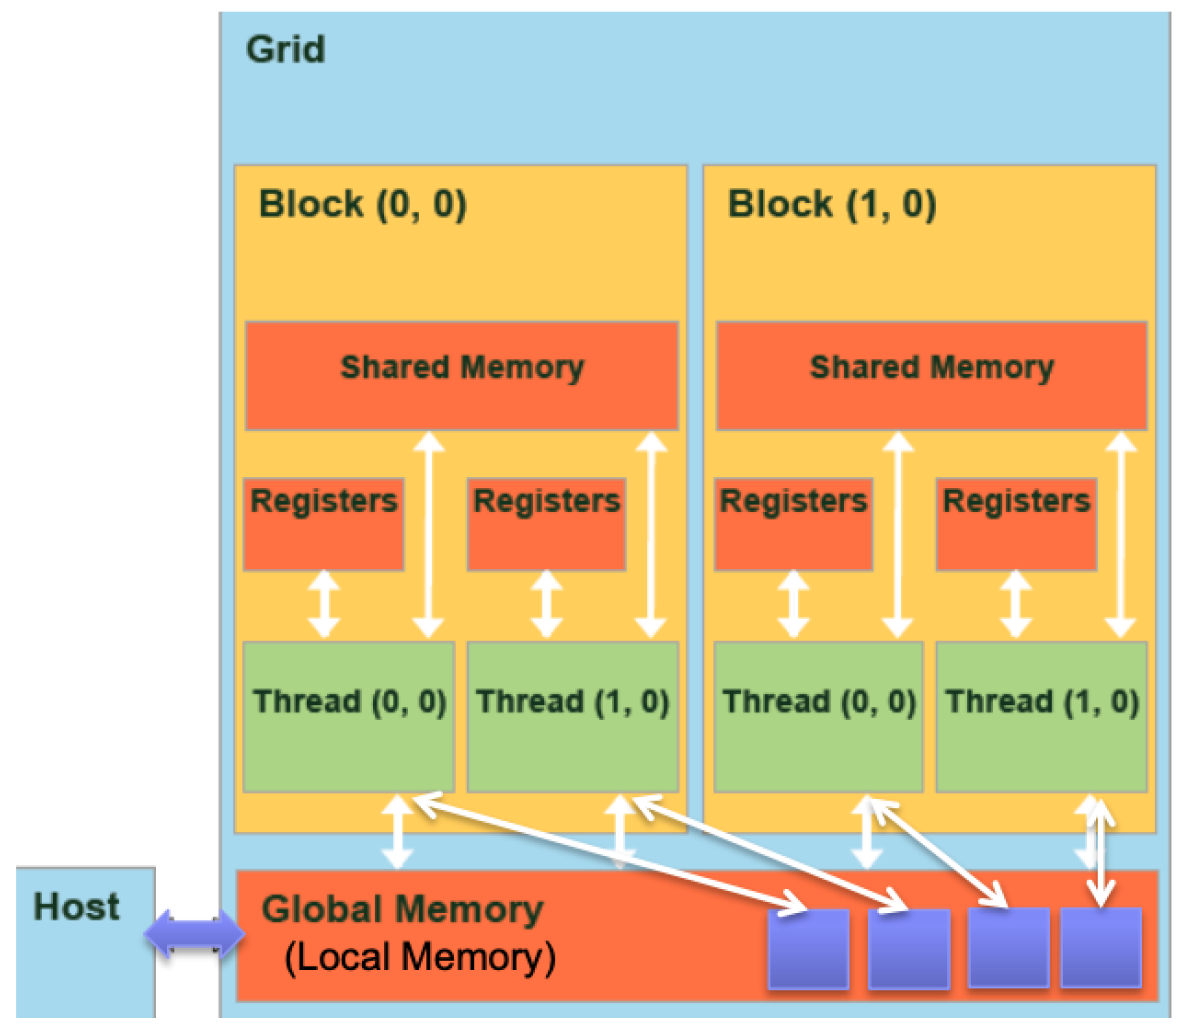
\includegraphics[width=11cm, keepaspectratio]{images/ch1/CUDA_memory_types_detailed.png}
	\caption{Different CUDA memory types visualized. Each thread has access to its local memory comprised of registers, local memory (blue squares in global memory), shared memory of its block, and global memory. Taken from Yao Hsiao's \emph{GPU - CUDA introduction} \cite{Hsiao17December2019}.}
	\label{Figure:CUDA-memory-types-detailed}
\end{figure}

Shared memory of each block is divided into 32-bit (4-byte) memory modules called words. A single word can store a float, half a double, 32-bit int, etc. - anything that can be stored in 32 bits. Apart from words, there are 32 banks per block. Each bank contains a number of words depending on the size of shared memory allocated. Since the size of shared memory can be up to 48 KB or more - depending on the version of CUDA Compute Capability - then the number of words per bank can differ between versions. Figure~\ref{Figure:CUDA-shared-memory-banks-words} visualizes the division of shared memory into banks and words.

\begin{figure}[h!]
	\centering
	\begin{subfigure}{\textwidth}
		\centering
		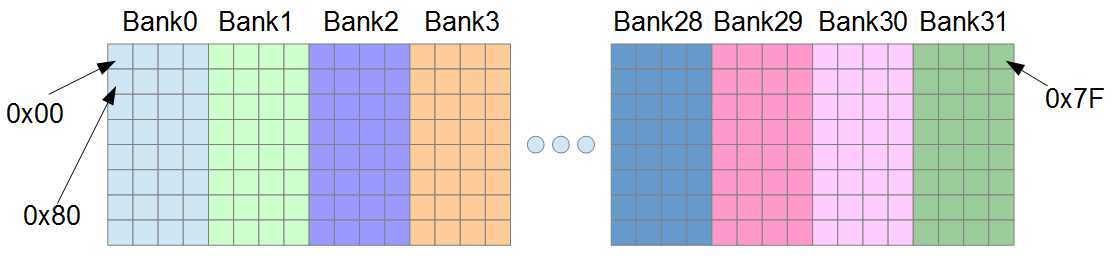
\includegraphics[width=14.5cm, keepaspectratio]{images/ch1/CUDA_shared_memory_banks_words.png}
		\subcaption{Shared memory divided into banks (columns under each \code{Bank*}), words (4 same-color squares of a row) and bytes (individual squares). In the first row, the first 4 bytes under \code{Bank0} - beginning at address \code{0x00} - make up the \code{0th} word (as show in Figure). The four bytes to the right of it (first row under \code{Bank1}) make up the \code{1st} word. Memory addresses of some bytes are shown hexadecimal.}
		\label{Figure:CUDA-shared-memory-banks-words-bytes}
	\end{subfigure}

	\begin{subfigure}{\textwidth}
		\centering
		\hspace*{-0.8cm}
		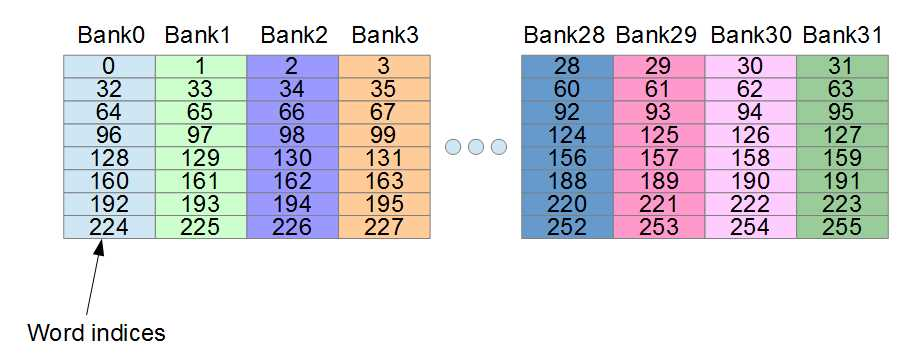
\includegraphics[width=13cm, keepaspectratio]{images/ch1/CUDA_shared_memory_banks_words_indices.png}
		\subcaption{Shared memory divided into banks (column under each \code{Bank*}) and words (individual rectangles with IDs inside).}
		\label{Figure:CUDA-shared-memory-banks-words-ids}
	\end{subfigure}
	\caption{Illustration of shared memory. In this example, there are 32 banks; each one has eight 4-byte (32-bit) words - in Figure~\ref{Figure:CUDA-shared-memory-banks-words-bytes} 1 byte is 1 square. Reading and writing into the \code{0th}, \code{32nd}, \code{64th}, etc. word is the responsibility of \code{Bank0}; reading and writing into the \code{1st}, \code{33rd}, \code{65th}, etc. word is the responsibility of \code{Bank1} and so on. Taken from \emph{Chapter 6: Shared Memory} of \emph{Cuda Succinctly} \cite{Rose2017}.}
	\label{Figure:CUDA-shared-memory-banks-words}
\end{figure}

Manipulating memory in banks can be fast and efficient under certain conditions. Let us consider the following example: Figure~\ref{Figure:CUDA-shared-memory-banks-words-ids} is the shared memory of a block that is used in a kernel. In this kernel, there is an array made up of 256 floats (32-bit) - each word in the figure is a single float. Furthermore, the IDs of words in the figure correspond to indices of floats in the array, thus, float values stored next to each other in memory belong to successive banks, for example, \code{arr[0]} belongs to \code{Bank0}, \code{arr[1]} belongs to \code{Bank1}, \code{arr[32]} belongs to \code{Bank0}, etc. \\
As mentioned by Chris Rose in \emph{CUDA Succinctly} \cite{Rose2017}, this division of words into banks is salient as each bank can serve only 1 word to a warp at once. This means that if a single word is requested from each bank, then all 32 threads of a warp can be served by all 32 banks simultaneously and expeditiously. Data serving is also fast when the same word from shared memory is accessed by all threads of a warp; this is called a \textit{broadcast} as shared memory is read once and the value is sent to all threads of the warp at once. \\
A concept similar to broadcasting is called a \textit{multicast}, which is an operation that is used when the same word from any particular bank is accessed by more than 1 thread of a warp. In this case, the threads that accessed the word will all receive it simultaneously from its bank. Under good conditions, the multicast operation is as fast as a broadcast. It is important to note that multicast is only available for compute capability 2.0 and higher. \\
However, the operations above all assumed good conditions for reading and writing of data. The primary originator of bad conditions for accessing shared memory is called a \textit{bank conflict}. Bank conflict describes an instance when threads of a warp request more than 1 word from any single bank. When this occurs, reading and writing of a word will be performed serially by the bank. For example - looking at Figure ~\ref{Figure:CUDA-shared-memory-banks-words-ids} - let thread \code{0} and thread \code{1} access words \code{0} and \code{32} respectively. Since both words belong to \code{Bank0}, then a bank conflict has occurred and the bank cannot distribute words' data in parallel. Instead, \code{Bank0} will firstly serve thread \code{0} with word \code{0} and then thread \code{1} with word \code{32}. \\
In order to facilitate further understanding, examples from \emph{Cuda succinctly} \cite{Rose2017} and \emph{CUDA C++ Programming Guide} \cite{NVIDIAMay2022} are included below. \\
Firstly, Table~\ref{Table:CUDA-shared-memory-access-patterns} presents different shared memory access patterns - including notes on the speed of execution. Then, Figure~\ref{Figure:CUDA-shared-memory-banks-words-no-conflicts} portrays shared memory access using random permutations, multicast and broadcast. Finally, Figure~\ref{Figure:CUDA-shared-memory-banks-words-conflicts} shows examples of strided shared memory access with and without bank conflict - additionally, this figure also visualizes some examples from Table~\ref{Table:CUDA-shared-memory-access-patterns}.

\begin{table}[h!]
	\centering
	\renewcommand{\arraystretch}{1.5}
	\begin{tabular}{ |l|l| } 
		\hline
		\textbf{Access Pattern} & \textbf{Notes} \\
		\hline
		\code{arr[0]}			& Fast - broadcast to all threads of the grid \\
		\hline
		\code{arr[bID]}			& Fast - broadcast to all threads of a block \\
		\hline
		\code{arr[tID]} 		& Fast - all threads request from different banks \\
		\hline
		\code{arr[tID/2]} 		& Fast - multicast; every 2 threads read from the same bank \\
		\hline
		\code{arr[tID*2]} 		& Slow - 2-way bank conflict \\
		\hline
		\code{arr[tID*3]} 		& Fast - all threads access different banks \\
		\hline
		\code{arr[tID*32]} 		& Egregiously slow - 32-way bank conflict \\
		\hline
	\end{tabular}
	\caption{Access patterns to shared memory. \code{arr} is an array stored in the shared memory of a thread block. \code{tID} is the ID of a thread and \code{bID} is the ID of a block. Taken from \emph{Chapter 6: Shared Memory} of \emph{Cuda Succinctly} \cite{Rose2017}.}
	\label{Table:CUDA-shared-memory-access-patterns}
\end{table}

\begin{figure}[h!]
	\centering
	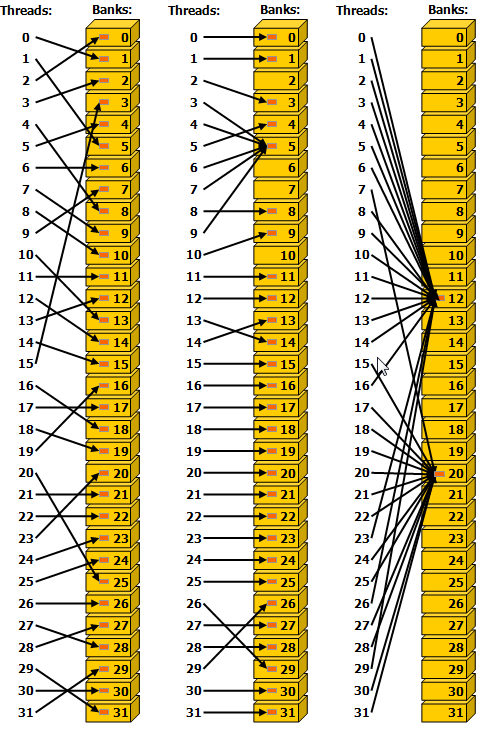
\includegraphics[width=11cm, keepaspectratio]{images/ch1/CUDA_shared_memory_banks_words_no_conflicts.png}
	\caption{Irregular shared memory accesses on 3 separate examples; yellow rectangular cuboids are banks; small orange rectangles are words. The left sub-image shows threads of a warp accessing shared memory randomly, however, in such a way that does not cause bank conflicts. The middle sub-image shows shared memory accessed by threads using the multicast operation, specifically, threads 3, 4, 5, 6, 7 and 9 accessing the same word from bank 5; other threads all access one word any bank each - no bank conflict. The right sub-image shows threads accessing shared memory via 2 broadcast operations. Taken from Nvidia's \emph{CUDA C++ Programming Guide} \cite{NVIDIAMay2022}.}
	\label{Figure:CUDA-shared-memory-banks-words-no-conflicts}
\end{figure}

\begin{figure}[h!]
	\centering
	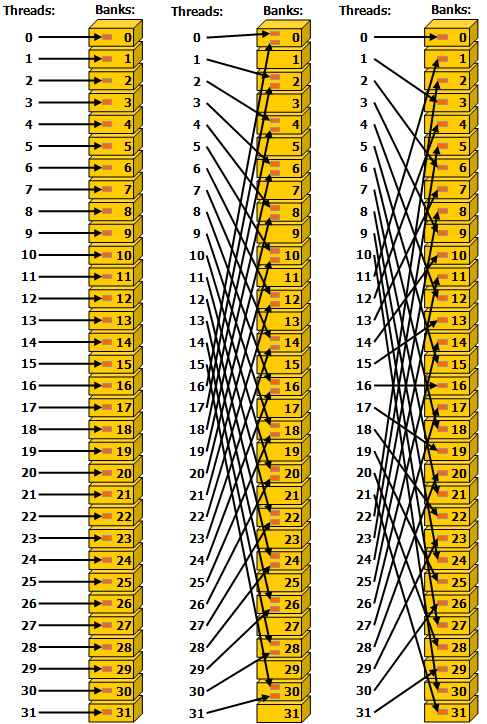
\includegraphics[width=11cm, keepaspectratio]{images/ch1/CUDA_shared_memory_banks_words_conflicts.png}
	\caption{Shared memory access using striding on 3 separate examples; yellow rectangular cuboids are banks; small orange rectangles are words. The left sub-image shows threads of a warp accessing shared memory with a stride of 1 (no bank conflict). The middle sub-image shows shared memory accessed by threads with a stride of 2 (equivalent to \code{arr[tID*2]} from Table~\ref{Table:CUDA-shared-memory-access-patterns}; 2-way bank conflict as threads access 2 different words from the same bank). The right sub-image shows threads accessing shared memory with a stride of 3 (equivalent to \code{arr[tID*3]} from Table~\ref{Table:CUDA-shared-memory-access-patterns}; no bank conflict). Taken from Nvidia's \emph{CUDA C++ Programming Guide} \cite{NVIDIAMay2022}.}
	\label{Figure:CUDA-shared-memory-banks-words-conflicts}
\end{figure}

In summary, ensuring that bank conflicts do not occur is pivotal to achieving efficient use of shared memory and subsequently high bandwidth.

\paragraph{Global memory}\label{Paragraph:CUDA-memory-management-global-memory}
The final, all-accessible memory layer is called \textit{global memory}. Some sources also refer to it as \textit{device memory} since global memory resides in the device's DRAM (Dynamic Random Access Memory) - not to be confused with the host's memory, often referred to as, RAM. The modifier 'global' represents the all-accessible aspect of this type of memory, as it can be accessed by the host and the device, thus, serving as a memory communication medium that can be used to transfer data between the two, and house input and output data for kernels \cite{Harris7January2013}. Global memory is available for all threads on the device, regardless of what thread structure they belong to. In other words, all grids have access to the same global memory - shown in Figure~\ref{Figure:CUDA-memory-management}.

\begin{figure}[h!]
	\centering
	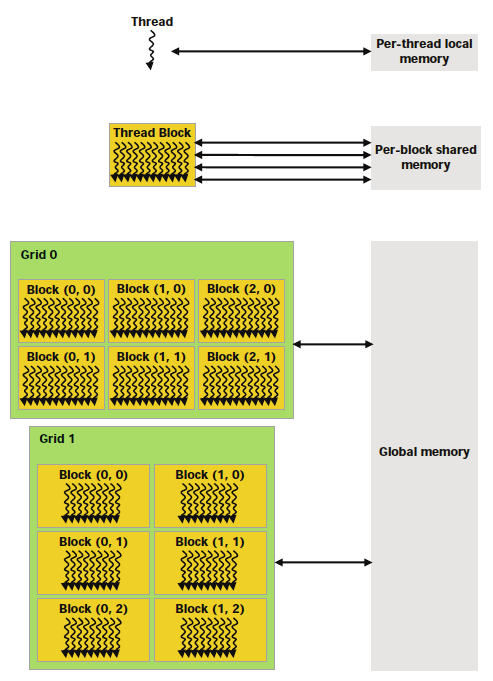
\includegraphics[width=11cm, keepaspectratio]{images/ch1/CUDA_memory_management.png}
	\caption{CUDA memory structuring. Taken from Nvidia's \emph{CUDA C++ Programming Guide} \cite{NVIDIAMay2022}.}
	\label{Figure:CUDA-memory-management}
\end{figure}

Unlike shared memory, global memory functions similarly to RAM: it is initialized with the startup of the program, it will be available while the program is running, and it is terminated with the termination of the program. In order to use global memory, the developer must manually allocate memory on the device, then copy the data from the host to the device, and finally, de-allocate (free) the data from the device \cite{Harris7January2013} once it is not required. \\
As mentioned above, in Paragraph~\emph{Per-thread local memory} in Subsection~\ref{Subsection:memory-management}, for the purpose of this project global memory is assumed to be off-chip - for completion, an exception to this is mentioned by Mark Harris in \emph{How to Access Global Memory Efficiently in CUDA C/C++ Kernels} \cite{Harris7January2013}: "\textit{Depending on the compute capability of the device, global memory may or may not be cached on the chip.}". Accessing (reading and writing) global memory is slower than accessing the aforementioned types of memory. In order to minimize this bottleneck, it is advised by Nvidia to keep the number of transactions that require accessing global memory to as few as possible \cite{Harris7January2013}. One of the main concepts that achieves this is called \textit{global memory coalesced access}. This methodology takes full advantage of the SIMD approach, specifically, instruction execution by threads in warps. In other words, it uses the fact that threads in a warp execute the same instruction simultaneously - in this instance: combine multiple memory accesses into a single transaction. \\
This means that upon the execution of a load instruction by all threads in a warp, the device will detect whether the threads are attempting to access successive global memory locations. If the accessed addresses are successive, then the accesses are coalesced (amalgamated) by the device into a consolidated access to consecutive DRAM locations \cite{Cabrera4December2019}. \\
More specifically, a single coalesced access into global memory - composed of a single access instruction performed by threads of a warp - occurs only if the following conditions are satisfied \cite{xUOrKLpxlGjvTonr, NVIDIAMay2022}:

\begin{enumerate}\label{Enumerate:CUDA-global-memory-coalesced-access-requirements}
	\item Each thread accesses a memory element of size 4, 8, or 16 bytes
	\item The device memory is accessed by memory transactions of 32, 64, or 128 bytes
	\item Each segment must be aligned to its size - first address is a multiple of their size
\end{enumerate}

The alignment requirement signifies that accessing (reading and writing) words of size 1, 2, 4, 8, or 16 bytes within global memory instructions is supported. Moreover, if the size of data stored in global memory is 1, 2, 4, 8, or 16 bytes and it is aligned, then access to this data is joined into 1 memory transaction. \\
Ad point 2 of the conditions above: when threads of a warp access words larger than 4 bytes, then the memory request made by the warp is divided into separate 128-byte memory requests. These newly-formed requests are subsequently performed separately, based on the word size \cite{NVIDIAMay2022}:

\begin{itemize}
	\item 8 bytes - 2 memory requests (1 for each half-warp)
	\item 6 bytes - 4 memory requests (1 for each quarter-warp)
\end{itemize}

Table~\ref{Table:CUDA-built-in-aligned-vector-types} shows examples of built-in vector types that are aligned in global memory by default; the entire list can be found in Nvidia's \emph{CUDA C++ Programming Guide} \cite{NVIDIAMay2022}.

\begin{table}[h!]
	\centering
	\renewcommand{\arraystretch}{1.5}
	\begin{tabular}{ |l|l| } 
		\hline
		\textbf{Type} & \textbf{Alignment} \\
		\hline
		int1, int2, int3, int4 & 4, 8, 4, 16 \\
		long1, long2, long3, long4 & 8, 16, 8, 16 \\
		float1, float2, float3, float4 & 4, 8, 4, 16 \\
		double1, double2, double3, double4 & 8, 16, 8, 16 \\
		\hline
	\end{tabular}
	\caption{Built-in vector types that are aligned by default. The suffix numbers specify the number of components the vector composes of, for example, a vector of type \code{int2} has 2 components: \code{(x, y)}. Taken from Nvidia's \emph{CUDA C++ Programming Guide} \cite{NVIDIAMay2022}.}
	\label{Table:CUDA-built-in-aligned-vector-types}
\end{table}

The size and alignment of other types, such as structures, must be approached manually: forcing the compiler to align them by using specifiers in code. For example, structures of 8 or 16 bytes that are to be aligned are declared using \code{\_\_align\_\_(8)} and \code{\_\_align\_\_(16)} respectively - shown in Listing~\ref{Listing:CUDA-aligned-structure-declaration}.

\begin{lstlisting}[caption={Declaration of to-be-aligned 8- and 16-byte structures. The lower example is aligned to 16 bytes as 12-byte alignment (3 4-byte floats) is not coalesced, therefore, 4 bytes are used for padding. Taken from Nvidia's \emph{CUDA C++ Programming Guide} \cite{NVIDIAMay2022}.},label={Listing:CUDA-aligned-structure-declaration}]
struct __align__(8) {
	float x;
	float y;
};

struct __align__(16) {
	float x;
	float y;
	float z;
};
\end{lstlisting}

On the other hand, if 8-byte or 16-byte words are not aligned, then reading them yields results offset by some words. \\
However, ultimately, if the size and alignment requirements are not adhered to, then the access to global memory is compiled into multiple instructions in such a way that they will not be fully coalesced, which leads to lower bandwidth and sub-optimal performance. \\
Examples of coalesced and non-coalesced memory accesses by a 16-thread warp are shown in Figures~\ref{Figure:CUDA-global-memory-coalesced-access} and \ref{Figure:CUDA-global-memory-non-coalesced-access-examples}.

\begin{figure}[h!]
	\centering
	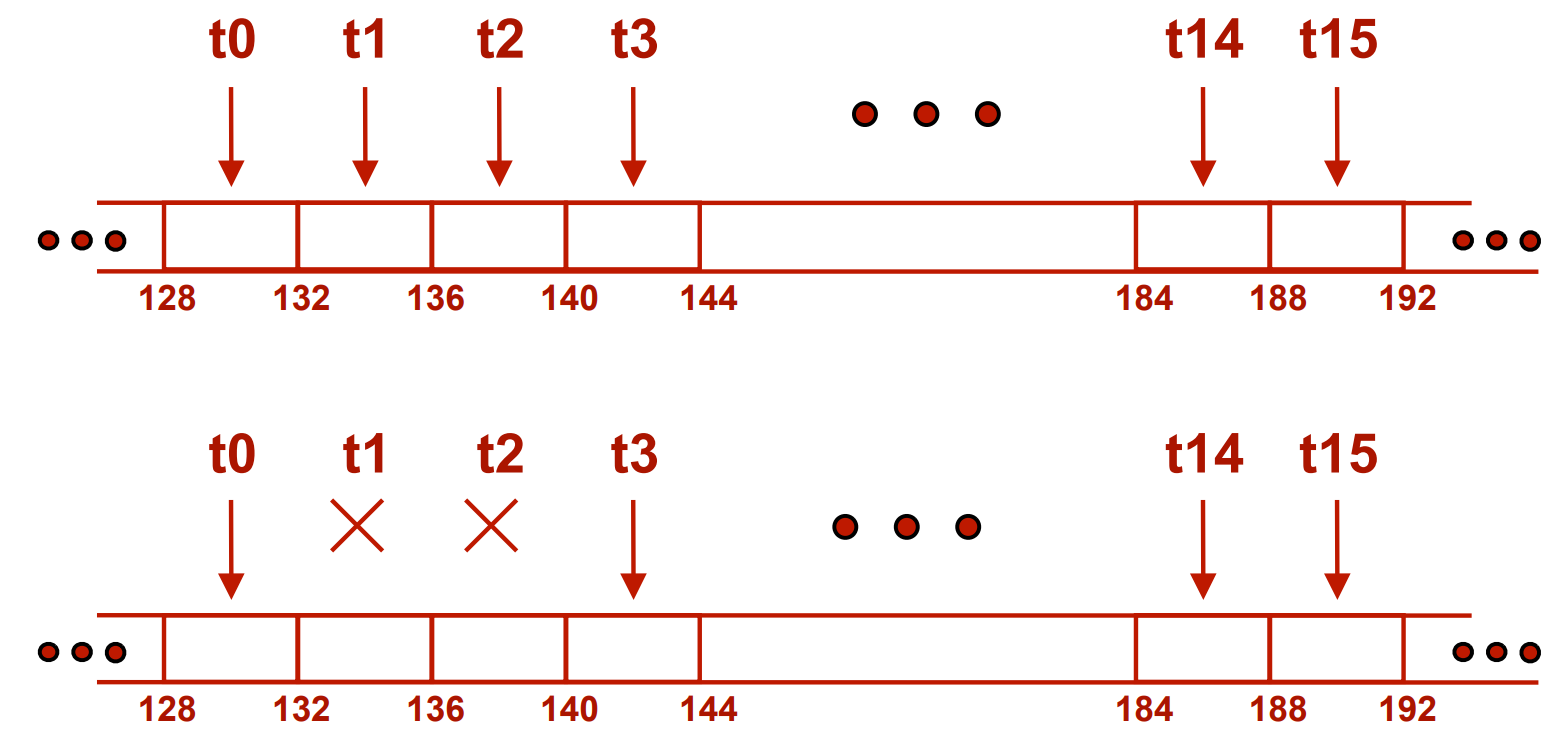
\includegraphics[width=0.7\textwidth, keepaspectratio]{images/ch1/CUDA_global_memory_coalesced_access.png}
	\caption{Coalesced access to global memory. Threads are denoted with \code{t<ID>} and the numbers below the rectangular memory locations are global memory addresses. In the upper image, all threads of the warp access successive memory addresses which house words of size 4 bytes (\code{float}), the size of the memory transaction is 64 bytes, and the segment is aligned to its size so that the first address is a multiple of its size: segment is 64 bytes and the starting address is 128: $ 128/64 = 2 $. The lower image shows an example where 2 threads from the 16-thread warp do not access data. Thus, threads of the warp have 2 separate execution paths (thread/warp divergence) that are executed sequentially. However, from a memory standpoint, the access is still coalesced as all requirements are fulfilled. Taken from Martínez Manuel Ujaldón's \emph{CUDA Optimizations, Debugging and Profiling} \cite{xUOrKLpxlGjvTonr}.}
	\label{Figure:CUDA-global-memory-coalesced-access}
\end{figure}

\begin{figure}[h!]
	\centering
	\begin{subfigure}{\textwidth}
		\centering
		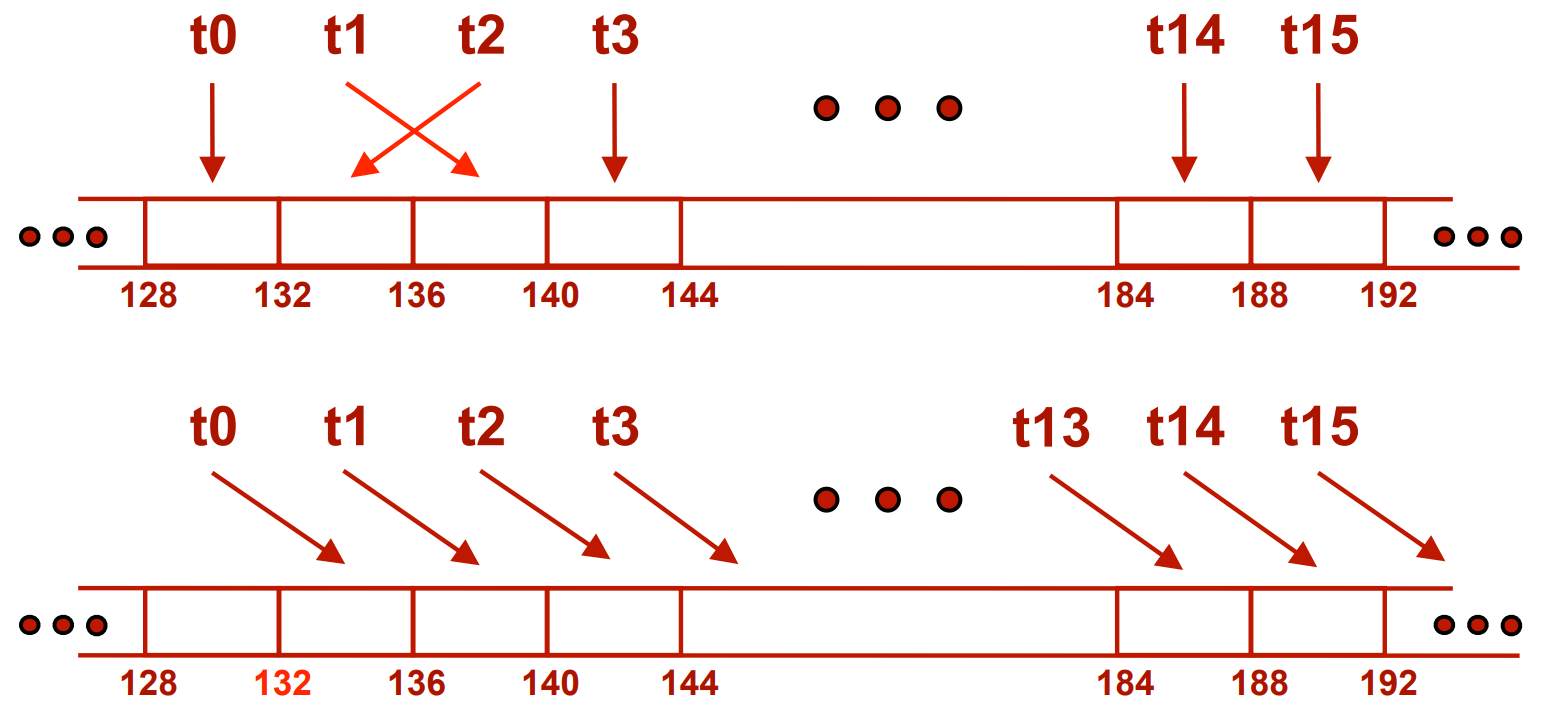
\includegraphics[width=0.7\textwidth, keepaspectratio]{images/ch1/CUDA_global_memory_non-coalesced_access.png}
		\subcaption{In the upper image, 2 threads swap orders and thus do not access successive floats in global memory. However, according to \emph{CUDA C++ Programming Guide} \cite{NVIDIAMay2022} this does not result in non-coalesced memory access. All other requirements are fulfilled. The lower image shows a scenario where the starting address is misaligned as the size of the memory segment is 64 bytes, but, the starting address is 132 which is not divisible by 64: $ 132/64 = 2.0625 $. Therefore, access is misaligned and the memory segment is read in 2 sequential memory transactions: starting addresses 128 - 188 and starting addresses 192-252.}
		\label{Sub-figure:CUDA-global-memory-non-coalesced-access}
	\end{subfigure}
	
	\begin{subfigure}{\textwidth}
		\centering
		\hspace*{-0.8cm}
		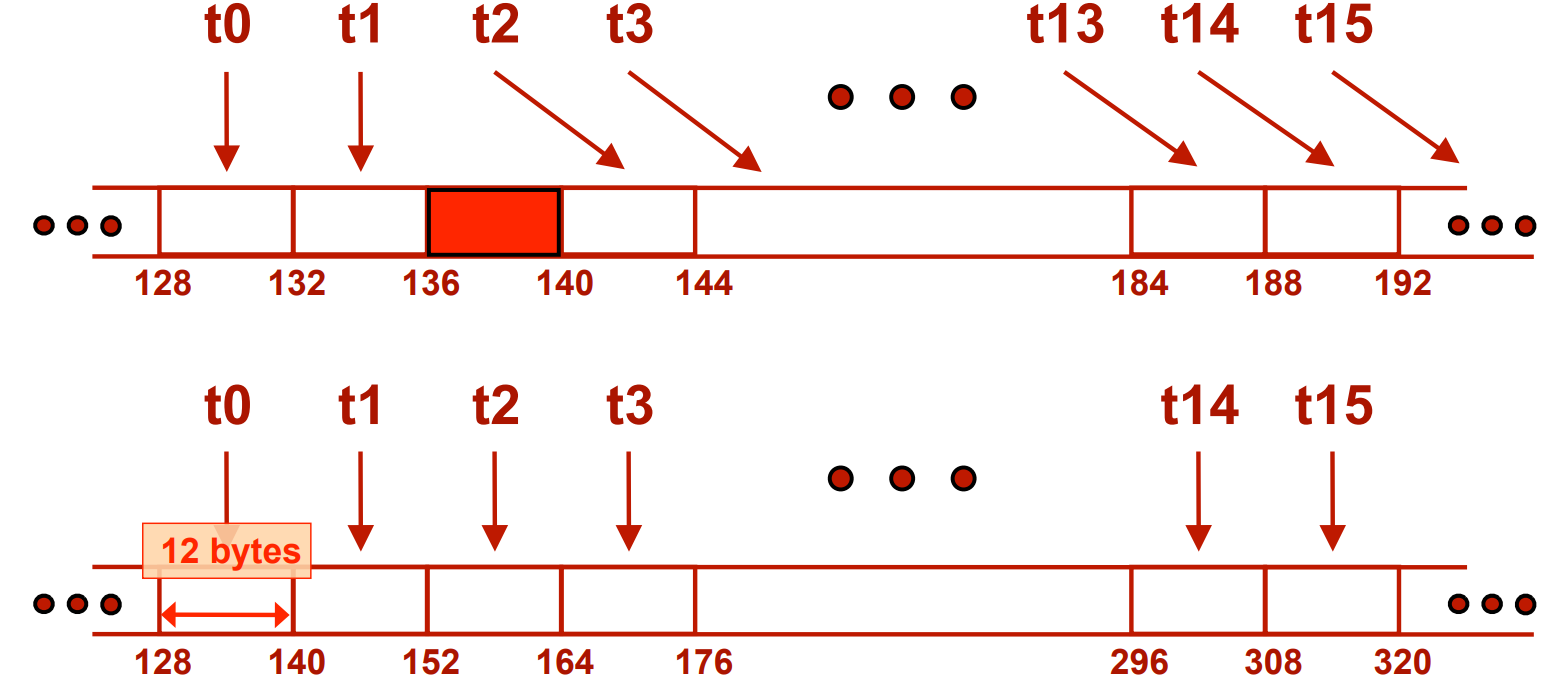
\includegraphics[width=0.7\textwidth, keepaspectratio]{images/ch1/CUDA_global_memory_non-coalesced_access-2.png}
		\subcaption{In the upper image, threads \code{t2} - \code{t15} are misaligned with the original starting address. Thus, similarly to the lower image in Sub-figure~\ref{Sub-figure:CUDA-global-memory-non-coalesced-access} the memory transaction will be split into 2 sequential transactions. The lower image shows a situation where global memory houses 12-byte \code{struct} types. However, as Table~\ref{Table:CUDA-built-in-aligned-vector-types} and Listing~\ref{Listing:CUDA-aligned-structure-declaration} show, 12-byte alignment is not supported and therefore global memory access is non-coalesced.}
		\label{Sub-figure:CUDA-global-memory-non-coalesced-access-2}
	\end{subfigure}
	\caption{Examples of coalesced and non-coalesced access to global memory composed of 4-byte words (for example, \code{float}) with 1 exception being 12-byte structures. Taken from Martínez Manuel Ujaldón's \emph{CUDA Optimizations, Debugging and Profiling} \cite{xUOrKLpxlGjvTonr}.}
	\label{Figure:CUDA-global-memory-non-coalesced-access-examples}
\end{figure}

In summary, coalesced access (reading and writing) to global memory must be fulfilled in order to not lower bandwidth - especially when dealing with custom non-built-in vector types - as global memory is implicitly high-latency and low-bandwidth compared to other memory types mentioned above.

\paragraph{Page-locked host memory}\label{Paragraph:CUDA-memory-management-page-locked-host-memory}
This type of memory that can be utilized within CUDA is different from the previous types in that it is not located on the device. Page-locked host memory - sometimes referred to as pinned - resides in the memory of the host. The difference between it and the host's regular pageable memory is its permanent placement and other properties related to CUDA. Firstly, it can be allocated and de-allocated using functions that come with CUDA: \code{cudaHostAlloc()} and \code{cudaFreeHost()}, or, if the memory on the host has already been allocated using \code{malloc()} it can be registered - made available within cuda - using \code{cudaHostRegister()}. According to \emph{CUDA C++ Programming Guide} \cite{NVIDIAMay2022} there are many advantages to using page-locked host memory:

\begin{itemize}
	\item Concurrent data transfer between page-locked host memory and device memory, and kernel execution - so-called \textit{asynchronous concurrent execution} (detailed in Subsection~\ref{Subsection:CUDA-asynchronous-concurrent-execution}).
	\item Elimination of data copying between the host and device by mapping page-locked host memory to the device's address space - so-called \textit{mapped memory} (detailed below).
	\item Higher bandwidth when copying between page-locked host memory and device memory on systems with a front-side bus. Furthermore, if the page-locked host memory is allocated using the write-combining principle, then bandwidth can be even higher.
\end{itemize}

Along with the above-mentioned advantages there are drawbacks such as, the small size of page-locked host memory. Since it is often used by the operating system for paging (host stores data - to-be-used in main memory - in paged memory on a drive rather than in RAM) it is not an abundant resource. Therefore, incautious use can lead to allocation failures and reduced system performance \cite{NVIDIAMay2022}.

\subparagraph{Mapped memory}
As mentioned above one of the advantages of using page-locked host memory is the ability to map this type of memory to the device's address space which eliminates the need for copying data stored in this memory between the host and the device. Specifically, a block of page-locked host memory can be mapped to the device's address space by passing either the \code{cudaHostAllocMapped} flag to \code{cudaHostAlloc()}, or, the \code{cudaHostRegisterMapped} flag to \code{cudaHostRegister()} \cite{NVIDIAMay2022}. \\
Then, the block will have an address in host memory - given by \code{cudaHostAlloc()} (or \code{malloc()}) - and another in device memory. The address in device memory is accessible by using the function \code{cudaHostGetDevicePointer()}, which will provide a pointer that can be used in kernels. Even though this specific type of host memory is accessible from within a kernel, it is not stored on the device and, thus, accessing it is not as fast as accessing device memory. \\
Another advantage of using mapped memory is that copying the block of data between device memory and mapped host memory is done implicitly by kernels when needed, thus, the need to allocate a block in device memory is removed. However, a disadvantage of this characteristic is the potential read-after-write, write-after-read, or write-after-write complications that can arise when asynchronous concurrent execution (detailed in Subsection~\ref{Subsection:CUDA-asynchronous-concurrent-execution}) is used \cite{NVIDIAMay2022}. These problems can be avoided by forcing memory synchronizations, however, this can have an impact on performance. \\
Further caveats associated with the use of mapped memory can be found in \emph{CUDA C++ Programming Guide} \cite{NVIDIAMay2022}.

\par An overview of how the structure of hardware on a GPU and CUDA can be seen in Figure~\ref{Figure:Nvidia-GPU-structure-CUDA-thread-structure}

\begin{figure}[h!]
	\centering
	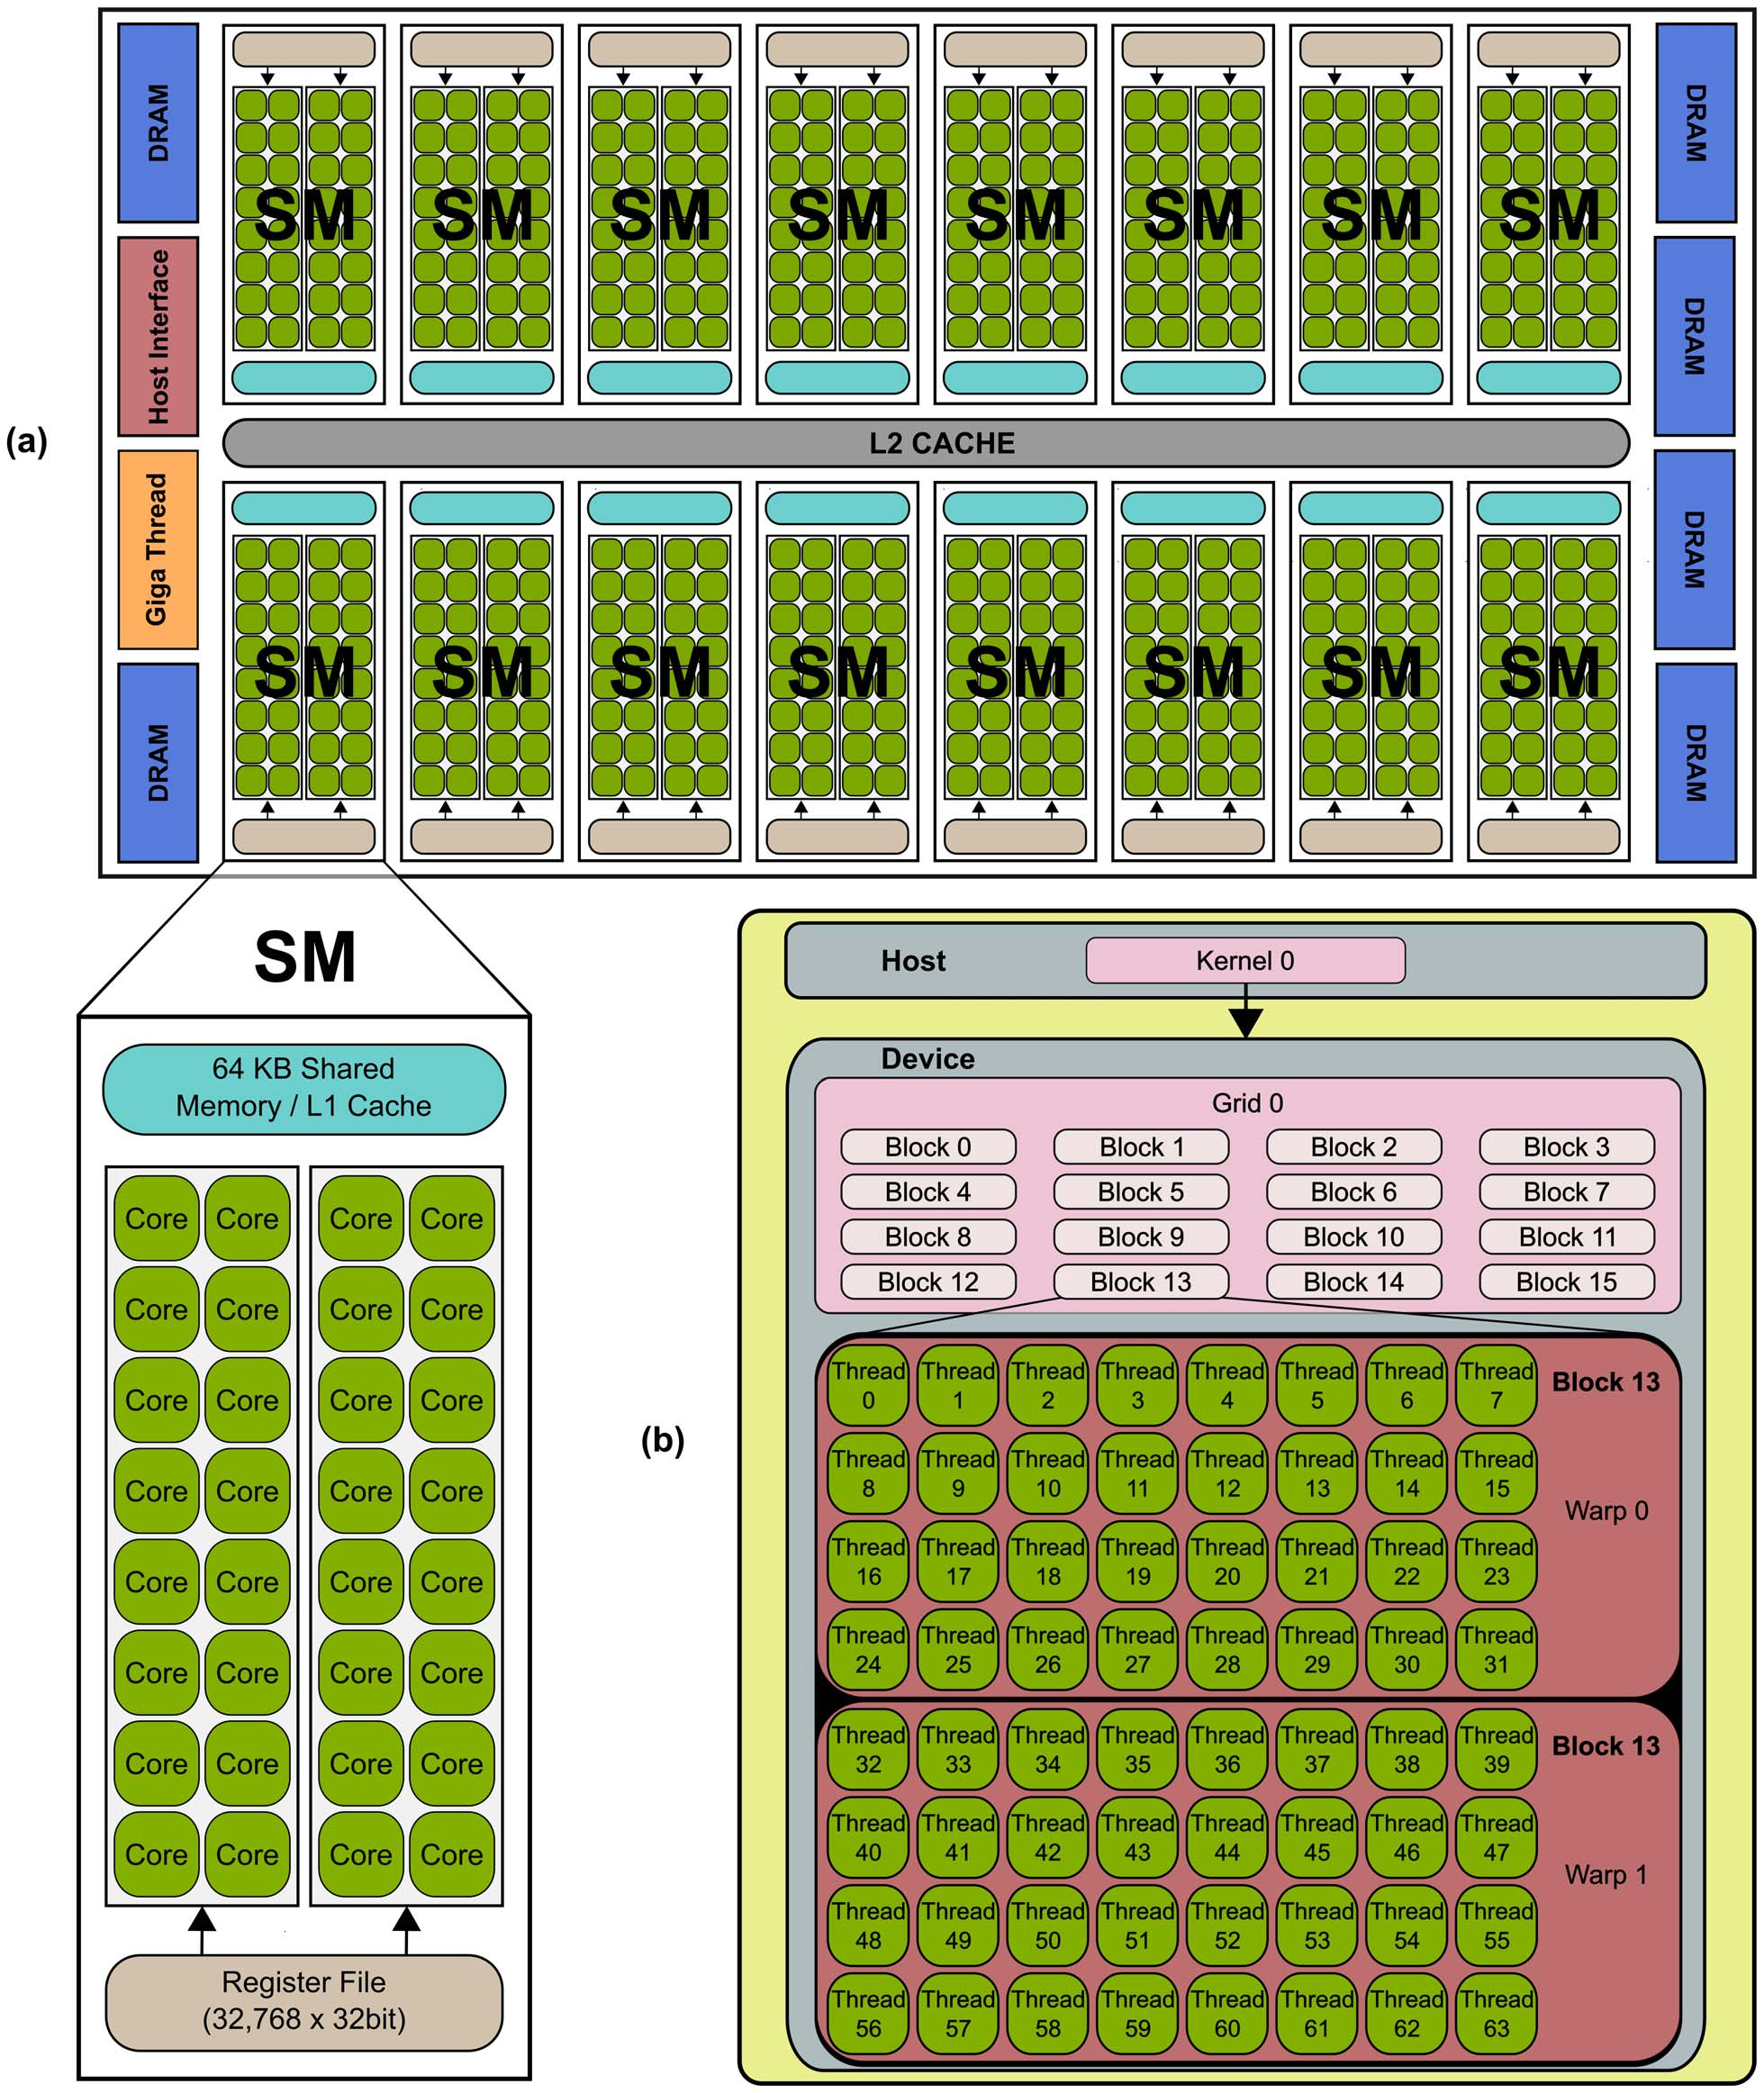
\includegraphics[width=\textwidth, keepaspectratio]{images/ch1/nvidia_gpu_sms_cuda.png}
	\caption{a) Usual architecture of an Nvidia Fermi GPU that comprises of SMs. Furthermore, each SM is made up of SP cores (Stream Processor cores) b) CUDA programming model controls the hardware of the GPU. Taken from \textit{Accelerating Fibre Orientation Estimation from Diffusion Weighted Magnetic Resonance Imaging Using GPUs} \cite{Hernandez2013429}.}
	\label{Figure:Nvidia-GPU-structure-CUDA-thread-structure}
\end{figure}

\subsection{Asynchronous concurrent execution \TO}\label{Subsection:CUDA-asynchronous-concurrent-execution}
Within CUDA there are multiple operations that can be executed at the same time (concurrently) - namely \cite{NVIDIAMay2022}:
\begin{itemize}
	\item Computation on the host
	\item Computation on the device
	\item Memory transfers from the host to the device and vice versa
	\item Memory transfers within the memory of a given device
\end{itemize}

However, it is important to note that there is a limit to concurrent load. According to \emph{CUDA C++ Programming Guide} \cite{NVIDIAMay2022} the so-called \textit{level of concurrency} is determined by the compute capability version of the device and its available feature set as detailed below. \\
This subsection will describe concurrent execution from different perspectives that are used in this project. Firstly, concurrent execution between the host and the device will be presented. Then, concurrent kernel execution will be introduced in greater detail and finally, the topic of streams will be described.
 
\paragraph{Concurrent execution between host and device}
Concurrent host execution means that once the host launches a kernel on the device, then it does not have to wait for the kernel to complete before moving on to the next instruction. CUDA has asynchronous library functions that make the host a controller which essentially sends computation jobs to the device. In other words, once a kernel is launched on the device, the host reclaims control immediately without waiting for the kernel to finish. This means that the host can go on to execute the next line of code. \\
Due to the asynchronous nature, this functionality is especially useful when it comes to queuing job for the device. The jobs are executed on the device by CUDA as soon as sufficient resources are available. Subsequently, the responsibility of managing the device is lifted from the host - allowing it to perform other tasks \cite{NVIDIAMay2022}. \\
Host asynchrony is available for the following device operations \cite{NVIDIAMay2022}:

\begin{itemize}
	\item Kernel launches
	\item Memory copies (only page-locked host memory):
	\begin{itemize}
		\item Within a single device's memory
		\item From host to device - memory block with a limited size of 64 KB
		\item Performed by functions suffixed with \code{Async}
	\end{itemize}
	\item Memory set function calls
\end{itemize}

Asynchronous concurrent execution between host and device can be disabled on a system for all CUDA applications (kernel launches) by using the \code{CUDA\_LAUNCH\_BLOCKING} environment variable (set to \code{1}). However, Nvidia does not recommend using this feature in production - only during debugging. \\
Another noteworthy aspect is that kernel launches are implicitly synchronous when running a CUDA application via a profiler, for example, the Nvidia Visual Profiler. This behavior can be overridden in the profiler by explicitly enabling concurrent kernel profiling \cite{NVIDIAMay2022}.

\paragraph{Concurrent kernel execution}\label{Paragraph:CUDA-asynchronous-concurrent-execution-concurrent-kernel-execution}
Similarly to the concept where the device can be running a kernel while the host is performing another task, kernels can be executed simultaneously on the device. Not all Nvidia devices support this functionality (only some devices with compute capability 2 and higher), therefore, it must be checked per-device using the \code{asyncEngineCount} device property (\code{0} if the device supports it). There are 3 main limitations when it comes to concurrent kernel execution: CUDA-defined maximum number of resident grids per device, no concurrent kernels from different CUDA contexts and resources available on the device. First, the CUDA-defined maximum resident grids per device will be explained. \\
Since each kernel is launched on an individual grid of blocks of threads, then the maximum number of resident grids per device is effectively the maximum number of kernels that can be run concurrently on the device. The limit is a hard-set constant that depends on the compute capability version - Table~\ref{Table:CUDA-maximum-resident-grids-per-device}.

\begin{table}[h!]
	\centering
	\renewcommand{\arraystretch}{1.5}
	\begin{tabular}{ |c|c|c|c|c|c|c|c|c| } 
		\hline
		Compute Capability & 3.5 - 5.2 & 5.3 & 6.0 & 6.1 & 6.2 & 7.0 & 7.2 & 7.5 - 8.7 \\
		\hline
		Max. resident grids per device & 32 & 16 & 128 & 32 & 16 & 128 & 16 & 128 \\
		\hline
	\end{tabular}
	\caption{Maximum number of resident grids per device depending on the CUDA compute capability version. Taken from Nvidia's \emph{CUDA C++ Programming Guide} \cite{NVIDIAMay2022}.}
	\label{Table:CUDA-maximum-resident-grids-per-device}
\end{table}

The second limitation - CUDA context - signifies that if there are two CUDA applications running at the same time on a system, then two kernels - one from each context - will not be run in concurrently. Instead, the kernel that was launched second will be queued to execute until the first kernel has finished. \\
The last limitation - device resources - is not as severe the previous 2 since kernels can still be launched concurrently, even if their cumulative required resources exceed the device's available resources. This is due to the fact that if more than 1 kernel is set to be launched concurrently, they are only run simultaneously if the available resources are sufficient for them all. If the resources available are not sufficient, then the kernels which would not get their requested resources are put aside until the resources are free. In this instance, resources represent memory and threads. \\
In terms of memory, an example of kernels that will often not run concurrently with other kernels are ones that require large amounts of local memory \cite{NVIDIAMay2022}. In terms of threads, the limiting factor is the maximum number of active threads - described at the end of the \textit{Grid} paragraph in Subsection~\ref{Paragraph:CUDA-thread-management-grid}. For example, if 2 kernels are to be run concurrently, the total number of threads required by them at once must not exceed the maximum number of active threads on the device. \\
Therefore, whether kernels can be run concurrently is highly dependent on the resource requirements of each kernel and it is up to the device to manage all of these operations.

\subsubsection{Streams \TO}\label{Subsubsection:CUDA-asynchronous-concurrent-execution-concurrent-streams}
Streams can be used to effectively create and manage concurrency on the device, in other words, they are the means by which the above-mentioned operations are controlled. According to \emph{CUDA C/C++ Streams and Concurrency} by Steve Rennich and Nvidia a CUDA \textit{stream} can be defined as "A sequence of operations that execute in issue-order on the GPU" \cite{sk7jHd5INXJOAEUe}. To put it another way, a single stream is basically an open door through which instructions can be sent to the device - kernels. \\
While it is possible to have multiple streams active at once, the device has limited resource available (active threads and memory). Therefore, multiple active streams at once does not necessarily mean multiple kernels running simultaneously. Nevertheless, if multiple streams are active and each is given a different kernel, then these kernels can be executed concurrently if the device's limits are not overstepped - detailed above in paragraph \textit{Concurrent kernel execution} in Section\ref{Paragraph:CUDA-asynchronous-concurrent-execution-concurrent-kernel-execution}. \\
Unlike individual kernels, global memory is used by all streams without division, i.e. all streams have access to the same global memory and there is no part of global memory that would belong to a particular stream. \\
According to Nvidia's \emph{CUDA C++ Programming Guide} \cite{NVIDIAMay2022}, individual streams are not dependent on each other, meaning that they are able to execute commands separately or concurrently. However, this behavior does not have to be consistent, for example, communication between kernels is not define. For this reason, Nvidia themselves recommend not relying on the accuracy of CUDA applications when attempting to make streams interact. \\
On the other hand, CUDA provides tools that can assist when synchronicity of streams is required. \\
This subsection will first present basic information on stream creation and destruction. Then, the topic of the default CUDA stream will follow and, finally, explicit and implicit synchronization will be detailed.

\paragraph{Creation and destruction}
A CUDA stream is created by initializing a stream object - type \code{cudaStream\_t} in code - and then creating the stream itself using \code{cudaStreamCreate()}. The approach that is often used in examples by Nvidia is to create an array of streams as shown in Listing~\ref{Listing:streams-creation}.

\begin{lstlisting}[caption={Creation of streams. Taken from Nvidia's \emph{CUDA C++ Programming Guide} \cite{NVIDIAMay2022}.},label={Listing:streams-creation}]
// Declare array of 2 stream objects
cudaStream_t streams[2];

// Create each stream
for (int i = 0; i < 2; ++i)
	cudaStreamCreate(&streams[i]);
\end{lstlisting}

In order to make a kernel run on a specific stream, the stream address must be specified as one of the launch parameters of the kernel - detailed in Subsection~\ref{Subsection:CUDA-C++-extensions}. Launching a kernel on a specific stream is shown in Listing~\ref{Listing:run-kernels-on-streams}.

\begin{lstlisting}[caption={Pseudo-code for launching 2 different kernels using 2 different streams. The instructions in this example would be executed from the host. Since each kernel is essentially an open door to the device for instructions, then, once \code{MyKernelA} is launched on \code{stream[0]}, the control is returned to the host without waiting for \code{MyKernelA} to finish. Subsequently, the host will immediately launch \code{MyKernelB} using \code{stream[1]}. In this example, each kernel is launched on a grid made up of 1 single-thread block with 0 bytes of dynamic shared memory allocated, thus, the devic resources will not be exhausted and both kernels will run concurrently. Taken from Nvidia's \emph{CUDA C++ Programming Guide} \cite{NVIDIAMay2022}.},label={Listing:run-kernels-on-streams}]
// Launch MyKernelA using the 0th stream using 1 block made up of 1 thread and 0 bytes of dynamically allocated shared memory
MyKernelA<<<1, 1, 0, stream[0]>>>(inputVariableA)

// Launch MyKernelB using the 1st stream
MyKernelB<<<1, 1, 0, stream[1]>>>(inputVariableB)
\end{lstlisting}

When streams are no longer needed, they are to be destroyed using \code{cudaStreamDestroy()} - show below in Listing~\ref{Listing:streams-destruction}. If \code{cudaStreamDestroy()} is called while a stream is still performing tasks, then it will return without destroying the stream immediately - the destruction (release) of the stream's resources will be delayed until all work is completed on the stream.

\begin{lstlisting}[caption={Destruction of streams. Taken from Nvidia's \emph{CUDA C++ Programming Guide} \cite{NVIDIAMay2022}.},label={Listing:streams-destruction}]
// Destroy each stream
for (int i = 0; i < 2; ++i)
	cudaStreamDestroy(stream[i]);
\end{lstlisting}

\paragraph{Default stream}\label{Paragraph:CUDA-asynchronous-concurrent-execution-streams-default-stream}
If a stream is not specified when launching a kernel, or when copying memory, then only the default stream - \textit{Stream '0'} - is used and the instruction are executed in order with respect to the device (not concurrently as shown in the examples above) \cite{NVIDIAMay2022}. \\
Nevertheless, it is possible to provide each host thread with its own default stream by setting the \code{---default-stream} compilation flag to \code{per-thread}, i.e. compiling using \code{nvcc ... ---default-stream per-thread}. \\
The default option for the flag is \code{legacy}, which signifies that all host threads will use the special \textit{NULL stream}. This stream is different from other streams as it uses implicit synchronization - detailed below in paragraph~\ref{Paragraph:CUDA-asynchronous-concurrent-execution-streams-implicit-synchronization}.

\paragraph{Explicit synchronization}
The first, and arguably the most used, type of synchronization when it comes to streams is explicit synchronization. In this instance, the 'explicit' modifier signifies that the synchronization is issued using one of the following functions from code \cite{NVIDIAMay2022, NvidiaJanuary2022}:
\begin{itemize}
	\item \code{cudaDeviceSynchronize()} - Synchronization of the entire device. This function servers as a checkpoint in code where streams will wait until they all get to this point in code.
	\item \code{cudaStreamSynchronize( cudaStream\_t stream )} - Synchronization of a particular stream. This function takes a single \code{stream} as its input parameter and serves a checkpoint to wait the for completion for all actions called before it.
	\item \code{cudaStreamWaitEvent(  cudaStream\_t stream, cudaEvent\_t event )} - Execution delayed for commands added to the input \code{stream} until the input \code{event} completes.
\end{itemize}

Additionally, CUDA provides a function to check whether all commands of a stream that precede the current line of code have finished: \code{cudaStreamQuery()}. Further functions that can be used to manage streams can be found in section \emph{6.4 Stream Management} in the \emph{CUDA Runtime API} \cite{NvidiaJanuary2022}.

\paragraph{Implicit synchronization}\label{Paragraph:CUDA-asynchronous-concurrent-execution-streams-implicit-synchronization}
The opposing type of synchronization is called implicit, and, as mentioned in paragraph \textit{Default stream} above, it is used by default under certain conditions - unless explicitly overridden by one of the functions above. Specifically, Nvidia states in \emph{CUDA C++ Programming Guide} \cite{NVIDIAMay2022} that if there are 2 streams, then 2 commands - each from 1 stream - cannot be run simultaneously if the host thread issues any of the following operations:

\begin{itemize}
	\item Page-locked host memory allocation
	\item Device memory allocation
	\item Device memory set
	\item Memory copy between 2 addresses to the same device memory
	\item Any CUDA command to the NULL stream
	\item Switch between the shared memory configurations
\end{itemize}

The hypothetical reasoning behind this is that if any of the operations above would be performed in parallel, it could create irresolvable conflicts. For example, if each stream tried to allocate memory on the device at the same location concurrently - impossible to be done in parallel without a conflict check. However, it can be argued that a conflict check is an unnecessary functionality as it is already present in some form when allocation happens sequentially. \\
Furthermore, there are certain operations that require a dependency check \cite{NVIDIAMay2022}:

\begin{itemize}
	\item Any other commands within the same stream as the launch being checked
	\item Any call to \code{cudaStreamQuery()} on that stream
\end{itemize}

Thus, in order to improve application performance, Nvidia recommends developers issue all independent operations before dependent operations and delay any synchronization until necessary.


\subsection{C++ CUDA Extensions \TO}\label{Subsection:CUDA-C++-extensions}
As previously mentioned at the beginning of Subsection~\ref{Section:CUDA}, CUDA supports a variety of programming languages. Among them is C++, a widely-used, high-performance C-based language that implicitly allows low-level memory manipulation. CUDA provides many different extensions to C++, however, for the purpose of this project only the core basics that were used during its development along with some other important extensions will be detailed. \\
This subsection will divided into 2 main categories: outer-kernel and inner-kernel extensions. The former is made up of memory-related operations (allocating, copying and freeing data), kernel launch configurations, function extensions, streams, etc. - i.e. extensions not used within kernels. The latter consists of any operators, structures and declarations that are used in kernels.

\subsubsection{Outer-kernel extensions}\label{Subsubsection:CUDA-C++-extensions-outer-kernel-extensions}
This category will first present a selection of important memory managing extensions along with those that were used during the development of this project. Then, kernel-specific extensions will be detailed. Finally, the last part will present function modifiers that state where a function can be executed. The extensions to C++ for streams were described above in the \textit{Streams} part of Subsection~\ref{Subsubsection:CUDA-asynchronous-concurrent-execution-concurrent-streams}.

\paragraph{Memory managing extensions}\label{Paragraph:CUDA-C++-extensions-outer-kernel-extensions-memory-managing-extensions}
CUDA offers many memory managing extensions to C++, however, there are a select few that are widely used for allocating, copying and freeing data \cite{NVIDIAMay2022, NvidiaJanuary2022, Cejka2020}:

\begin{itemize}
	\item \code{cudaMalloc( void** devPtr, size\_t size )} - Function that allocates \code{size} bytes in device memory and stores the address in the \code{devPtr} pointer. \\
	Note that since the pointer is to an address located in device memory, it is inaccessible from the host - access from the host would first require for the data to be copied using \code{cudaMemcpy()}. \\
	This function is widely used when it comes to allocating anything from single variables to large arrays. \\
	If the data was allocated successfully, then \code{cudaSuccess} is returned, otherwise one of \code{cudaErrorInvalidValue}, \code{cudaErrorMemoryAllocation} is returned - depending on the type of failure.
	\item \code{cudaMemcpy( void* dst, const void* src, size\_t count, }\\ \code{cudaMemcpyKind kind )} - Function that copies \code{count} bytes from the source memory address (\code{src}) to the destination memory address (\code{dst}). The \code{kind} parameter specifies the direction of copying; it has to be one of the following: \code{cudaMemcpyHostToHost}, \code{cudaMemcpyHostToDevice}, \code{cudaMemcpyDeviceToHost}, \code{cudaMemcpyDeviceToDevice}, or \code{cudaMemcpyDefault}. \\
	Similarly to \code{cudaMalloc()}, if the data was copied successfully, then \code{cudaSuccess} is returned, otherwise one of \code{cudaErrorInvalidValue}, \\ \code{cudaErrorInvalidMemcpyDirection} is returned - depending on the type of failure.
	\item \code{cudaFree( void* devPtr )} - Function that frees memory on the device that is pointed to by \code{devPtr}. \\
	If the memory was successfully freed, then \code{cudaSuccess} is returned, otherwise \code{cudaErrorInvalidValue} is returned. \\
	It is also worth noting that in order to be freed using \code{cudaFree()} the memory \code{devPtr} is pointing to must have been allocated by one of CUDA's memory allocation APIs, for example, \code{cudaMalloc()}, \code{cudaMallocAsync()}, etc. - the complete list can be found in Nvidia's \emph{CUDA Runtime API: API Reference Manual} \cite{NvidiaJanuary2022}.
	\item \code{cudaMallocHost( void** ptr, size\_t size )} - Function that allocates \code{size} bytes of page-locked memory on the host and stores the address in the \code{ptr} pointer. The benefits and caveats of using page-locked memory are detailed in paragraph \textit{Page-locked host memory} in Subsection~\ref{Paragraph:CUDA-memory-management-page-locked-host-memory}.
\end{itemize}

Expanding on the memory operations mentioned above, CUDA provides memory space specifiers that can be used to denote in what memory a variable ought to be stored. Among such often-used specifiers are \cite{NVIDIAMay2022}:

\begin{itemize}
	\item \code{\_\_device\_\_} - Memory space specifier declaring that a variable is stored in global memory on the device. Since it resides in global memory, it is accessible by all threads from the grid and it is present for the lifetime of the CUDA application. It is noteworthy that if multiple CUDA devices are present in the system, then a variable with this specifier is a unique object for each device.
	\item \code{\_\_shared\_\_} - Memory space specifier declaring that a variable is stored in shared memory of a thread block. Since it resides in shared memory, it is only accessible by threads of a block as each block has its own unique object of this variable.
\end{itemize}

Listing~\ref{Code:CUDA-memory-managing-extensions-example} shows an example of how memory managing functions can be used in a host-device code that copies arrays.

\begin{lstlisting}[caption= Example of code that utilizes CUDA memory managing extensions of C++. Taken from \textit{Formats for storage of sparse matrices on GPU} \cite{Cejka2020} and Nvidia's \emph{Getting Started with CUDA} presentation \cite{Ruetsch2008}.,label=Code:CUDA-memory-managing-extensions-example]
	int main(void)
	{
		float *a_h, *b_h; // data that will be allocated on host
		float *a_d, *b_d; // data that will be allocated on device
		int N = 14, nBytes, i;
		
		nBytes = N * sizeof( float ); // required allocation size
		a_h = (float *) malloc( nBytes ); // allocating host data
		b_h = (float *) malloc( nBytes ); 
		cudaMalloc( (void **) &a_d, nBytes ); // allocating device data
		cudaMalloc( (void **) &b_d, nBytes );
		
		// filling up host data
		for( i = 0, i < N; i++ ) a_h[ i ] = 100.f + i;
		
		// copying data from host -> device -> device -> host
		cudaMemcpy( a_d, a_h, nBytes, cudaMemcpyHostToDevice );
		cudaMemcpy( b_d, a_d, nBytes, cudaMemcpyDeviceToDevice );
		cudaMemcpy( b_h, b_d, nBytes, cudaMemcpyDeviceToHost );
		
		// checking that all data is equal
		for( i = 0; i < N; i++ ) assert( a_h[ i ] == b_h[ i ] );
		
		free( a_h ); free( b_h ); // freeing data on host
		cudaFree( a_d ); cudaFree( b_d ); // freeing data on device
		return 0;
	}
\end{lstlisting}

\paragraph{Kernels}
While the term \textit{kernel} was introduced earlier in Subsection \ref{Subsection:CUDA-introductory-terminology}, the technical details will be covered in this part. In order to differentiate a kernel from a function, the \code{\_\_global\_\_} modifier must be used. Another distinction that kernels have compared to regular functions is the kernel launch configuration which has the following specific syntax: \code{$<$$<$$<$ numBlocks, threadsPerBlock, sharedMemSize,} \code{stream $>$$>$$>$} where \cite{NVIDIAMay2022, Cejka2020}:

\begin{itemize}
	\item \code{numBlocks} specifies the number of blocks in the grid and their structure;
	\item \code{threadsPerBlock} specifies the number of threads per block and their structure;
	\item \code{sharedMemSize} specifies the number of bytes that are to be dynamically allocated in shared memory for each block (on top of any statically allocated shared memory). This argument is not mandatory and its default value is 0;
	\item \code{stream} specifies stream to which the kernel should be sent for execution. This argument is also not mandatory and defaults to 0 - the default stream.
\end{itemize}

The \code{sharedMemSize} parameter is of type \code{size\_t}, \code{stream} is of type \code{cudaStream\_t}, and parameters \code{numBlocks} and \code{threadsPerBlock} can be either of type \code{int} or \code{dim3}. The \code{dim3} type is a 3-dimensional \code{unsigned int} vector used to specify dimensions. It can be defined with up to 3 variables (1 for each dimension) with an implicit dimension value of 1, i.e., if a vector component (dimension) is not specified when declaring a \code{dim3} variable, it is by default initialized to 1. \\
For example, if \code{numBlocks} is of type \code{int}, then the grid is one-dimensional and composed of \code{numBlocks} blocks. Concordantly, if \code{threadsPerBlock} is type \code{int}, then all blocks in the grid will be one-dimensional with \code{threadsPerBlock} threads. \\
On the other hand if \code{threadsPerBlock} is a \code{dim3} variable, then the thread structure of all blocks can be up to three-dimensional. An example of a kernel being called with the properties above can be seen in Listing~\ref{Listing:CUDA-kernel-example}.

\begin{lstlisting}[caption={Example of C++ pseudocode of a Kernel launch on a grid consisting of 1 one-dimensional block that is made up of 8 threads. Taken from Nvidia's \emph{CUDA C++ Programming Guide} \cite{NVIDIAMay2022}.},label={Listing:CUDA-kernel-example}]
// Kernel definition
__global__ void MyKernel(float a, float b, float c)
{
	// Kernel code here
}

int main()
{
	...
	// Kernel invocation on a grid with 1 block of 8 * 1 * 1 threads
	int numBlocks = 1;
	dim3 threadsPerBlock(8); // Defaults to (8, 1, 1)
	MyKernel<<<numBlocks, threadsPerBlock>>>(a, b, c);
	...
}
\end{lstlisting}

\paragraph{Function extensions}
In the part above, the \code{\_\_global\_\_} modifier was introduced as a specifier for functions that are to be considered kernels. Along with it, CUDA brings other function modifiers, or, as Nvidia calls them: \textit{execution space specifiers} \cite{NVIDIAMay2022}:

\begin{itemize}
	\item \code{\_\_global\_\_} - Modifier declaring that a function can be called from both the host and the device (as of compute capability 3.2 or higher). However, it can only be executed on the device. Additionally, a function denoted with this modifier must not belong to any class and it can only have a void return type. Furthermore, the launch configuration mentioned above in the \textit{Kernels} paragraph must be specified for each call.
	\item \code{\_\_device\_\_} - Modifier declaring that a function can only be called from and executed on the device. This means that it can only be called from within kernels.
	\item \code{\_\_host\_\_} - Modifier declaring that a functions can only be called from and executed on the host. This means that it can only be called from regular functions, not kernels.
\end{itemize}

If no modifier is included for a function, it is compiled for the host only. However, if both \code{\_\_device\_\_} and \code{\_\_host\_\_} are specified for a function, then it is compiled both for the host and for the device. The complete list of modifiers can be found in \emph{CUDA C++ Programming Guide} \cite{NVIDIAMay2022}.

\subsubsection{Inter-kernel extensions \TO}
This category comprises of variables, structures and operations etc. that are most often used within a kernel. First, the means by which developers are able to identify individual threads will be detailed. Then, different memory-type identifiers will be briefly presented along with established operations used to avoid erroneous behaviors in kernels.

\paragraph{Thread identification}
Once a kernel is a launched on the device, it can be run concurrently on thousands of threads. This presents a scenario where the developer must distinguish what each thread will perform within the kernel. For this purpose, the following variables - among others - are available within every kernel for each thread \cite{NVIDIAMay2022}:

\begin{itemize}
	\item \code{threadIdx} - ID of a thread within a block stored in a 3-component vector (1 component for each of 3 dimensions). For example, if the thread block is 2-dimensional, then \code{threadIdx.x} stores the thread's ID in the first dimension and \code{threadIdx.y} stores the thread's ID in the second dimension - the pair of IDs is unique only within the thread's block.
	\item \code{blockIdx} - ID of a block within a grid stored in a 3-component vector (1 component for each of 3 dimensions). Similarly to \code{threadIdx}, the block's ID in the first dimension is retrieved using \code{blockIdx.x}, the second using \code{blockIdx.y} and the third using \code{blockIdx.z}. Within a kernel, the block ID refers to the block of threads that the executing thread belongs to.
	\item \code{blockDimx} - Dimensions of a thread's block stored in a 3-component vector (1 component for each of 3 dimensions). For example, for a block made up of \code{32x16x2} threads: \code{blockDimx.x = 32}, \code{blockDimx.y = 16} and \code{blockDimx.z = 2}.
\end{itemize}

The variables above can be combined to calculate the global ID of a thread, i.e. the thread's ID within a grid:
$$\code{globalID = blockIdx.x * blockDimx.x + threadIdx.x}$$
The \code{globalID} is useful when working with matrices, for example, adding 2 matrices. In such an example, each thread would take 2 elements (1 from each matrix), add them and then store the result into a new matrix - as shown in Listing~\ref{Listing:CUDA-matrix-addition-example}.

\begin{lstlisting}[caption={Example of C++ pseudocode of a kernel that adds 2 matrices using 2-dimensional thread blocks. Since each thread has a unique \code{globalID} for each of 2 dimensions, then those IDs can be used as indices for adding matrix elements. This simple example does not take into account allocation and copying data from host to device. Taken from Nvidia's \emph{CUDA C++ Programming Guide} \cite{NVIDIAMay2022}.},label={Listing:CUDA-matrix-addition-example}]
// Kernel definition
__global__ void MatAdd(float A[N][N], float B[N][N], float C[N][N])
{
	// Get thread ID for each dimension -> use as matrix indices
	int i = blockIdx.x * blockDim.x + threadIdx.x;
	int j = blockIdx.y * blockDim.y + threadIdx.y;
	
	// Check if the IDs are within the dimensions of the matrices
	if (i < N && j < N)
		C[i][j] = A[i][j] + B[i][j];
}

int main()
{
	...
	// Number of threads per each 2-dimensional block is 16x16 = 256
	dim3 threadsPerBlock(16, 16);
	
	// Number of blocks in the grid depends on the matrix dimension (NxN)
	dim3 numBlocks(N / threadsPerBlock.x, N / threadsPerBlock.y);
	
	// Kernel launch: A + B = C
	MatAdd<<<numBlocks, threadsPerBlock>>>(A, B, C);
	...
}
\end{lstlisting}

Accompanying the code in Listing~\ref{Listing:CUDA-matrix-addition-example}, Figure~\ref{Figure:CUDA-GridBlockThread-Structure} visualizes how elements of a matrix can be divided into a grid comprising of 2-dimensional thread blocks.

\begin{figure}[h!]
	\centering
	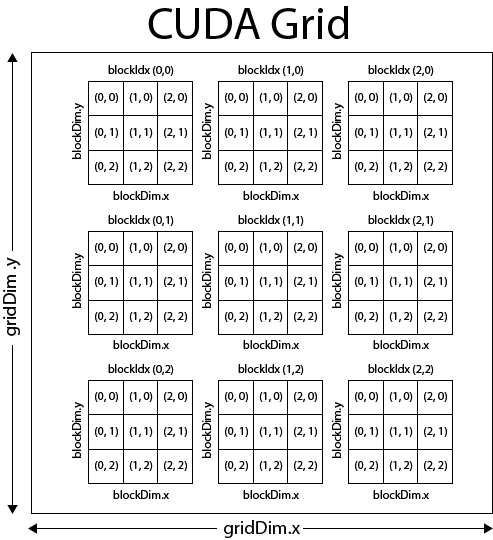
\includegraphics[width=0.8\textwidth, keepaspectratio]{images/ch1/CUDA-GridBlockThread-Structure.png}
	\caption{Grid made up of 2-dimensional thread blocks. Each square represents a thread with its IDs within its block (\code{threadIdx.x}, \code{threadIdx.y}). It can be imagined that each block is a sub-matrix and together all sub-matrices make up the full matrix. Taken from \emph{CUDA Parallel Thread Management} \cite{McKennon13June2013}.}
	\label{Figure:CUDA-GridBlockThread-Structure}
\end{figure}

Finally, as mentioned in paragraph \textit{Global memory} in Subsection~\ref{Paragraph:CUDA-memory-management-global-memory}, the coalesced access of threads effectively means that neighboring threads access global memory. To add to this, it is important to mention that threads are considered neighboring in the first dimension. In other words, neighbors according to \code{threadIdx.x} values.

\paragraph{Memory specifiers and other operations}
Some memory space specifiers described in above in paragraph \textit{Memory managing extensions} in Subsection~\ref{Paragraph:CUDA-C++-extensions-outer-kernel-extensions-memory-managing-extensions} can be used within kernels, specifically the \code{\_\_shared\_\_} specifier. Its use within kernels is mostly related to statically allocated shared memory where the size of the variable or array is known during compilation \cite{NVIDIAMay2022}. An example showing this use of the specifier can be seen in Listing~\ref{Listing:CUDA-matrix-multiplication-with-shared-memory-example}. \\
In paragraph \textit{Shared memory} in Subsection~\ref{Paragraph:CUDA-memory-management-shared-memory}, it was mentioned that threads of a block are able to share data purely among each other. However, this advantage can also bring problems, such as, some threads overwriting data that other threads have not finished using, or, some threads reading data that other threads have not yet written - known as a \textit{race condition} \cite{Harris28January2013}. CUDA addresses this issue by enabling the synchronization of threads in a block which can be done by calling the built-in function: \code{\_\_syncthreads()}. This function can seen as a meeting checkpoint for all threads of a particular block, i.e., threads of a block will wait at this point until every single thread in their block has finished their work until this point. To put it more clearly: threads of a block are halted on the the line in code that contains \code{\_\_syncthreads()} until all threads of the block arrive to at it \cite{NVIDIAMay2022}.


\subsection{Matrix multiplication \TO}\label{Subsection:matrix-multiplication}
In order to consolidate how CUDA can be used to accelerate the execution of a simple task, such as matrix multiplication, this subsection will present solutions to this task from Nvidia's \emph{CUDA C++ Programming Guide} \cite{NVIDIAMay2022}. Furthermore, for the purpose of showcasing and stressing the importance of abiding by Nvidia's recommendations when it comes to best practices and optimal performance, 2 examples will be presented. The first example will only use global memory to read the input matrix and write the resulting matrix, i.e. without shared memory. On the other hand, the second example will use shared memory to minimize accessing global memory. \\
It is important to note that neither example is fully functional as the logic of some functions has been omitted due to unnecessary complexity and irrelevance to showcasing the capabilities of CUDA. In other words, the code shown will not compile, nor will it run - the full code can be found in Nvidia's \emph{CUDA C++ Programming Guide} \cite{NVIDIAMay2022}. The full working example (\code{matrixMul.cu}) encompassed by the build automation tool \code{make} can be unpacked during the installation of a CUDA toolkit. \\
Before introducing the specifics of each example, their similarities will be presented. \\
First, the task that will be performed is matrix multiplication:

\begin{equation}\label{Equation:matrix-multiplication-definition}
	\mathbb{C} = \mathbb{A} \cdot \mathbb{B}
\end{equation}

In the context of this operation all matrix dimensions are assumed such that it is a legal operation. Additionally, for simplicity, the dimensions of the matrices are assumed to be multiples of the thread block size. This limitation can be avoided by allocating an extra row and column of blocks in the grid and setting a boundary condition in the kernel - each of the 2 examples (global vs shared memory) require slightly different approaches which will be described later. \\
Let each matrix be represented by a structure \code{Matrix}:

\begin{lstlisting}[caption={Definition of the structure that will represent a matrix. The \code{width} variable stores the number of columns and \code{height} stores the number of rows the matrix has. The elements of the matrix are stored in row-major order in the single-precision (float) array: \code{values}. Taken from Nvidia's \emph{CUDA C++ Programming Guide} \cite{NVIDIAMay2022}.},label={Listing:CUDA-matrix-multiplication-matrix-structure-definition}]
// Matrices are stored in row-major order:
// M(row, col) = *(M.values + row * M.width + col)
typedef struct {
	int width;
	int height;
	float* values;
} Matrix;
\end{lstlisting}

Furthermore, let there be a host function \code{MatMul} that will:

\begin{enumerate}
	\item Take matrices $ \mathbb{A} $, $ \mathbb{B} $, $ \mathbb{C} $ from Equation~\ref{Equation:matrix-multiplication-definition} as input structures: \code{A}, \code{B}, \code{C}.
	\item Allocate memory for the matrix structures on the device.
	\item Copy the matrix structures from host to device memory.
	\item Invoke the matrix multiplication kernel with a constant thread block size set at compile time.
	\item Copy the resulting matrix from device to host memory.
	\item Free previously allocated memory from the device.
\end{enumerate}

Listing~\ref{Listing:CUDA-matrix-multiplication-host-mat-mul-function} shows the implementation of the points mentioned above.

\begin{lstlisting}[caption={Definition of the function that will allocate and copy all matrices to the device, invoke the kernel and then free the device memory. The size of the thread block is constant and set during compile time using the \code{\#define} macro. Taken from Nvidia's \emph{CUDA C++ Programming Guide} \cite{NVIDIAMay2022}.},label={Listing:CUDA-matrix-multiplication-host-mat-mul-function}]
// Thread block size - 16x16 = 256 threads
#define BLOCK_SIZE 16

// Matrix multiplication - Host code
// Matrix dimensions are assumed to be multiples of BLOCK_SIZE
void MatMul( const Matrix A, const Matrix B, Matrix C )
{
	// Allocate and copy A to device memory
	Matrix d_A;
	d_A.width = A.width; d_A.height = A.height;
	size_t size = A.width * A.height * sizeof(float);
	cudaMalloc( &d_A.values, size );
	cudaMemcpy( d_A.values, A.values, size, cudaMemcpyHostToDevice );
	
	// Allocate and copy B to device memory
	Matrix d_B;
	d_B.width = B.width; d_B.height = B.height;
	size = B.width * B.height * sizeof(float);
	cudaMalloc( &d_B.values, size );
	cudaMemcpy( d_B.values, B.values, size, cudaMemcpyHostToDevice );
	
	// Allocate C in device memory
	Matrix d_C;
	d_C.width = C.width; d_C.height = C.height;
	size = C.width * C.height * sizeof(float);
	cudaMalloc( &d_C.values, size );
	
	// Invoke kernel
	dim3 threadPerBlock( BLOCK_SIZE, BLOCK_SIZE );
	dim3 numBlocks( B.width / threadPerBlock.x, A.height / threadPerBlock.y );
	MatMulKernel<<< numBlocks, threadPerBlock >>>( d_A, d_B, d_C );
	
	// Read C from device memory
	cudaMemcpy( C.values, d_C.values, size, cudaMemcpyDeviceToHost );
	
	// Free device memory
	cudaFree( d_A.values );
	cudaFree( d_B.values );
	cudaFree( d_C.values );
}
\end{lstlisting}

The \code{Matrix} structure and \code{MatMul} function conclude the equivalent part of the examples.

\subsubsection{Example without shared memory \TO}
The first example uses only global memory access, i.e. without shared memory. This means that the kernel - invoked on line 31 in Listing~\ref{Listing:CUDA-matrix-multiplication-host-mat-mul-function} - receives the \code{Matrix} structures stored in global memory and each thread reads from and writes to the same global memory whenever they need to. \\
The kernel is launched on a grid of thread such that each thread is responsible for calculating exactly 1 element of the resulting \code{C} matrix. For example, let there be a thread with indices \code{row\_id} and \code{col\_id}. This thread will perform element-wise multiplication of row \code{row\_id} from matrix \code{A} and column \code{col\_id} from matrix \code{B}. Then, it will store the sum of these elements as the resulting value \code{C(row\_id, col\_id)} into matrix \code{C}. \\
The visualization of this approach is shown in Figure~\ref{Figure:CUDA-matrix-multiplication-without-shared-memory-example} and the kernel is presented in Listing~\ref{Listing:CUDA-matrix-multiplication-without-shared-memory-example}.

\begin{figure}[h!]
	\centering
	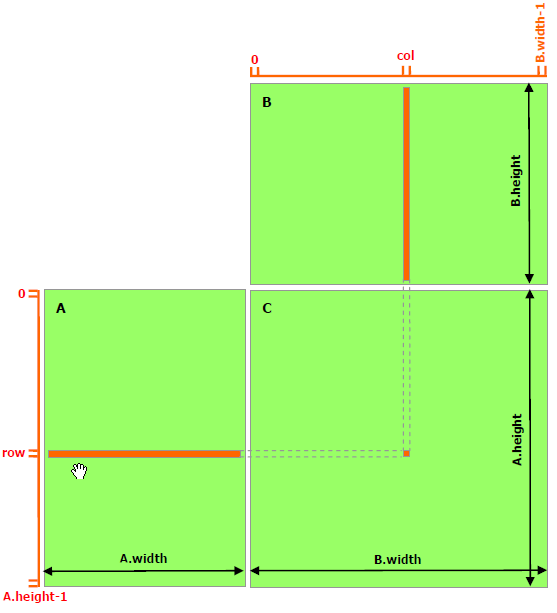
\includegraphics[width=0.8\textwidth, keepaspectratio]{images/ch1/CUDA-matrix-multiplication-without-shared-memory.png}
	\caption{Visualization of the execution of the kernel that does not use shared memory - shown in Listing~\ref{Listing:CUDA-matrix-multiplication-without-shared-memory-example}. Taken from Nvidia's \emph{CUDA C++ Programming Guide} \cite{NVIDIAMay2022}.}
	\label{Figure:CUDA-matrix-multiplication-without-shared-memory-example}
\end{figure}

\begin{lstlisting}[caption={Definition of the matrix multiplication kernel that uses global memory without shared memory. Each thread has a variable \code{Cvalue} stored in registers into which it calculates its specific \code{C(row, col)} matrix element. Taken from Nvidia's \emph{CUDA C++ Programming Guide} \cite{NVIDIAMay2022}.},label={Listing:CUDA-matrix-multiplication-without-shared-memory-example}]
// Matrix multiplication kernel called by MatMul()
__global__ void MatMulKernel( Matrix A, Matrix B, Matrix C )
{
	// Each thread computes one element of C by accumulating results into Cvalue
	float Cvalue = 0;
	int row = blockIdx.y * blockDim.y + threadIdx.y;
	int col = blockIdx.x * blockDim.x + threadIdx.x;
	for( int i = 0; i < A.width; ++i )
		Cvalue += A.values[row * A.width + i] * B.values[i * B.width + col];
	
	C.values[row * C.width + col] = Cvalue;
}
\end{lstlisting}

As can be seen in Listing~\ref{Listing:CUDA-matrix-multiplication-without-shared-memory-example}, each thread performs \code{A.width + B.height} reads from global memory when calculating its \code{Cvalue}. Since CUDA threads are executed simultaneously in a warp of 32 threads, the memory access to global memory should be coalesced for the threads within each warp. Nevertheless, this kernel is sub-optimal as accessing global memory is considered sub-optimal when avoidable.
\par At the end of the introduction to Subsection~\ref{Subsection:matrix-multiplication}, it was mentioned that in order to eliminate the "matrix dimensions being multiples of \code{BLOCK\_SIZE}" requirement, the kernel would need to include a boundary condition. In this example, the condition would be simply to allocate an extra column and row of thread blocks to the grid. This would mean that the last row and column of blocks would overlap the dimensions of the matrix. Then, the kernel would be terminated for threads that are outside the matrix dimensions, i.e. if either \code{row} is greater than \code{A.height} or \code{col} is greater than \code{B.width}. However, it is noteworthy that this will result in thread divergence, even though in this instance it will not have a large impact on overall performance as one of the execution paths would be a simple \code{return} statement.

\subsubsection{Example with shared memory \TO}
The second example uses both global and shared memory. Similarly to the approach without using shared memory, each thread is responsible for calculating a single element of the resulting \code{C} matrix. However, in this example, each thread is also responsible for loading elements of matrices \code{A} and \code{B} from global memory into shared memory. Thus, shared memory is the primary means of obtaining elements for calculations. Overall, the calculation is changed from each thread calculating its individual element to a block of threads iterating over sub-matrices of \code{A} and \code{B}. \\
\par In order to make use of shared memory, matrix \code{C} is divided into sub-matrices of \code{BLOCK\_SIZE x BLOCK\_SIZE} elements ($ \mathbb{C}_{sub} $). Then, each sub-matrix $ \mathbb{C}_{sub} $ is computed by a single thread block; each thread within a thread block is responsible for the computation of an element in $ \mathbb{C}_{sub} $. In the previous approach, each thread performed element-wise multiplication of a row and a column to form a resulting element of matrix \code{C} - effectively a multiplication of an \code{1xn} and \code{nx1} matrix. The approach with shared memory expands this concept to blocks. In other words, the sub-matrix $ \mathbb{C}_{sub} $ is a result of multiplying 2 rectangular sub-matrices of \code{A} and \code{B} (illustrated in Figure~\ref{Figure:CUDA-matrix-multiplication-with-shared-memory-example}) - denoted $ \mathbb{A}_{rect} $ and $ \mathbb{B}_{rect} $ for the purpose of this explanation:

\begin{enumerate}
	\item $ \mathbb{A}_{rect} $ is a \code{BLOCK\_SIZE x A.width} sub-matrix of \code{A} that has the same row indices as $ \mathbb{C}_{sub} $.
	\item $ \mathbb{B}_{rect} $ is a \code{B.height x BLOCK\_SIZE} sub-matrix of \code{B} that has the same column indices as $ \mathbb{C}_{sub} $.
\end{enumerate}

\begin{figure}[h!]
	\centering
	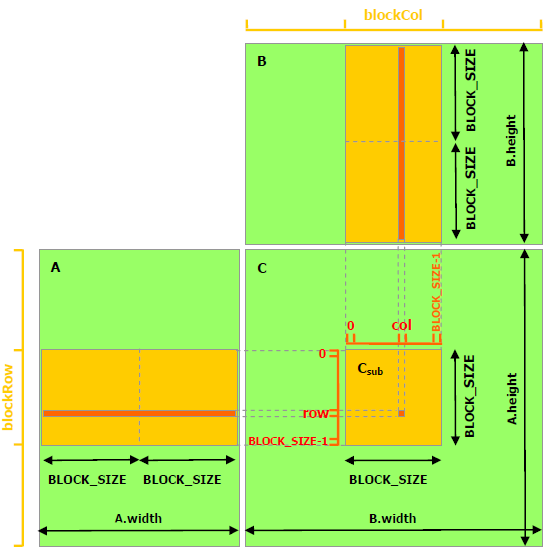
\includegraphics[width=0.8\textwidth, keepaspectratio]{images/ch1/CUDA-matrix-multiplication-with-shared-memory.png}
	\caption{Visualization of the execution of the kernel that uses shared memory - shown in Listing~\ref{Listing:CUDA-matrix-multiplication-with-shared-memory-example}. Taken from Nvidia's \emph{CUDA C++ Programming Guide} \cite{NVIDIAMay2022}.}
	\label{Figure:CUDA-matrix-multiplication-with-shared-memory-example}
\end{figure}

The rectangular sub-matrices $ \mathbb{A}_{rect} $ and $ \mathbb{B}_{rect} $ are split into \code{BLOCK\_SIZE x BLOCK\_SIZE} sub-matrices $ \mathbb{A}_{sub} $ and $ \mathbb{B}_{sub} $. A thread block will begin its computation by multiplying the leftmost $ \mathbb{A}_{sub} $ with the uppermost $ \mathbb{B}_{sub} $, then it will move to the next $ \mathbb{A}_{sub} $ on the right and to the next $ B_{sub} $ below. After every iteration, each thread appends its partial sum to the \code{Cvalue} variable that it is responsible for in the $ \mathbb{C}_{sub} $ sub-matrix. The computation of $ \mathbb{C}_{sub} $ is finished once the thread block reaches and multiplies the rightmost $ \mathbb{A}_{sub} $ and the lowermost $ \mathbb{B}_{sub} $ sub-matrix. \\
The reasoning behind splitting $ \mathbb{A}_{rect} $ and $ \mathbb{B}_{rect} $ into multiple $ \mathbb{A}_{sub} $ and $ \mathbb{B}_{sub} $ respectively stems from the use of shared memory in every iteration for a particular block:

\begin{enumerate}
	\item All threads of the block load $ \mathbb{A}_{sub} $ and $ \mathbb{B}_{sub} $ from global memory to a two-dimensional array residing in the block's shared memory.
	\item Each thread of the block performs its computation, i.e. it multiplies row \code{row\_id} from\space $ \mathbb{A}_{sub} $ with column \code{col\_id} from$ \mathbb{B}_{sub} $ and sums the resulting values (\code{row\_id} and \code{col\_id} are the thread's IDs).
	\item Each thread stores the temporary result to its local variable \code{Cvalue} stored in its registers.
	\item If there still is a $ \mathbb{A}_{sub} $ to the right and a $ \mathbb{B}_{sub} $ below, then, all threads of the block move to them and continue to step 1.
	\item Otherwise, the computation is finished and all threads store their local variable \code{Cvalue} to the element that they're responsible  in $ \mathbb{C}_{sub} $ that resides in global memory.
\end{enumerate}

The visualization of this approach is shown in Figure~\ref{Figure:CUDA-matrix-multiplication-with-shared-memory-example} and the kernel is presented in Listing~\ref{Listing:CUDA-matrix-multiplication-with-shared-memory-example}.

\begin{lstlisting}[caption={Definition of the matrix multiplication kernel that uses both global memory with shared memory. The \code{GetSubMatrix(mtx, row, col)} is a function returns a \code{BLOCK\_SIZE x BLOCK\_SIZE} sub-matrix of a matrix that is located \code{col} sub-matrices to the right and \code{row} sub-matrices down from the upper-left corner of a the specified \code{Matrix}. The \code{GetElement(sub\_mtx, row, col, val)} function returns the element found at a matrices \code{row} and \code{col} indices. Taken from Nvidia's \emph{CUDA C++ Programming Guide} \cite{NVIDIAMay2022}.},label={Listing:CUDA-matrix-multiplication-with-shared-memory-example}]
// Matrix multiplication kernel called by MatMul()
__global__ void MatMulKernel( Matrix A, Matrix B, Matrix C )
{
	// Block row and column - indices of the sub-matrices within A and B respectively
	int blockRow = blockIdx.y;
	int blockCol = blockIdx.x;
	
	// Each thread block computes one sub-matrix Csub of C
	Matrix Csub = GetSubMatrix( C, blockRow, blockCol );
	
	// Each thread computes one element of Csub by accumulating results into Cvalue
	float Cvalue = 0;
	
	// Thread row and column within Csub
	int row = threadIdx.y;
	int col = threadIdx.x;
	
	// Loop over all the sub-matrices of A and B that are required to compute Csub by multiplying each pair of sub-matrices together and accumulate the results
	for( int i = 0; i < (A.width / BLOCK_SIZE); ++i ) {
		
		// Get sub-matrix Asub of A
		Matrix Asub = GetSubMatrix( A, blockRow, i );
		
		// Get sub-matrix Bsub of B
		Matrix Bsub = GetSubMatrix( B, i, blockCol );
		
		// Shared memory used to store Asub and Bsub respectively
		__shared__ float As[BLOCK_SIZE][BLOCK_SIZE];
		__shared__ float Bs[BLOCK_SIZE][BLOCK_SIZE];
		
		// Load Asub and Bsub from device memory to shared memory
		// Each thread loads one element of each sub-matrix
		As[row][col] = GetElement( Asub, row, col );
		Bs[row][col] = GetElement( Bsub, row, col );
		
		// Synchronize to make sure the sub-matrices are loaded before starting the computation
		__syncthreads();
		// Multiply Asub and Bsub together
		for( int k = 0; k < BLOCK_SIZE; ++k )
			Cvalue += As[row][k] * Bs[k][col];
		
		// Synchronize to make sure that the preceding computation is done before loading two new sub-matrices of A and B in the next iteration
		__syncthreads();
	}
	
	// Write Csub to device memory - each thread writes one element
	SetElement( Csub, row, col, Cvalue );
}
\end{lstlisting}

Unlike the previous example, the code shown in Listing~\ref{Listing:CUDA-matrix-multiplication-with-shared-memory-example} has less accesses to global memory which leads to an performance improvement as detailed later in the \textit{Comparison of examples} part of Subsection~\ref{Subsubsection:matrix-multiplication-comparison-of-examples}. Concretely, in the kernel above, each thread performs only \code{A.width/BLOCK\_SIZE + B.height/BLOCK\_SIZE} reads from global memory when loading sub-matrices $ \mathbb{A}_{sub} $ and $ \mathbb{B}_{sub} $ into shared memory. This means that all threads will perform \code{BLOCK\_SIZE} times less accesses to global memory and \code{A.width + B.height} accesses to shared memory instead. Equivalently to the example before, the access to global memory is coalesced. Thus, by Nvidia's recommendations, this kernel can be considered being close to optimal.

\par In order to eliminate the "matrix dimensions being multiples of \code{BLOCK\_SIZE}" requirement, the kernel would need to include a boundary condition. In the earlier approach it was a matter of allocating extra blocks and terminating the kernel for threads that would reach out of matrix bounds. However, for this approach - with shared memory - that method would result in incorrect results as the threads that would reach out of bounds for one matrix read elements into shared memory from the other matrix. Thus, the boundary condition is split into:

\begin{enumerate}
	\item If the thread would reach out of bounds of a particular matrix, load the edge element, i.e. the last element of the row/col before the thread would reach out of bounds. This condition would be used when the elements are being loaded from global into shared memory.
	\item Then let the computation continue as normal - to avoid thread divergence of threads.
	\item Once the computation si done, terminate the threads that would reach out of bounds of matrix \code{C} before they write their results to global memory.
\end{enumerate}

This solution ensures correct results and avoids a case of thread divergence in the main loop which would occur multiple times during the computation. However, the thread divergence will still occur when deciding which value to load from global memory and when terminating the kernel for some threads. Nevertheless, similarly to the previous approach, in this instance thread divergence will not have a large impact on overall performance as one of the execution paths would be a simple assignment operation in the first condition and a \code{return} statement in the second condition.

\subsubsection{Comparison of both examples \TO}\label{Subsubsection:matrix-multiplication-comparison-of-examples}
In order to show the performance difference, benchmarks for both examples using single precision were run on a set of matrices with varying dimensions - from 160 by 160 to 16000 by 16000. The hardware and software specifications of the machine used for the benchmarks can be found in Table~\ref{Table:CUDA-matrix-multiplication-benchmark-system}. Furthermore, the full code can be found in Attachment~\ref{Attachment:CUDA-matrix-multiplication-code}.

\begin{table}[h]
	\centering
	\begin{tabular}{|l|l|}
		\hline
		CPU              & Ryzen 9 5900x @ 3.7 GHz (12 cores, 24 threads) \\
		RAM              & 32GB RAM \\
		GPU              & Nvidia GeForce GTX 1070 8GB GDDR5 (256.3 GByte/s)\\
		Operating System & Ubuntu 20.04.4 LTS (Focal Fossa) \\
		Compiler         & GCC 8.4.0 \\
		CUDA             & CUDA 11.5 \\ \hline
	\end{tabular}
	\caption{Specifications of the platform that the matrix multiplication benchmarks were run on.}
	\label{Table:CUDA-matrix-multiplication-benchmark-system}
\end{table}

The operation measured during the benchmark was only the multiplication of matrices
$$ \mathbb{C} = \mathbb{A} \cdot \mathbb{B} $$
In other words, allocation and copying of the matrices was not included in the measurement. Furthermore, the operation was looped 10 times - the measured FLOPS and run times were averaged from the 10 recorded loops. The values in Matrix $ \mathbb{A} $ were all set to $ 1 $ and to $ 0.1 $ in matrix $ \mathbb{B} $. The benchmark results in FLOPS can be found in Figure~\ref{Figure:CUDA-matrix-multiplication-benchmark-results-flops} and Table~\ref{Table:CUDA-matrix-multiplication-benchmark-results-msec} shows the results in milliseconds.

\begin{figure}
	\centering
	\tikzset{mark options={mark size=2.5, line width=1pt}}
	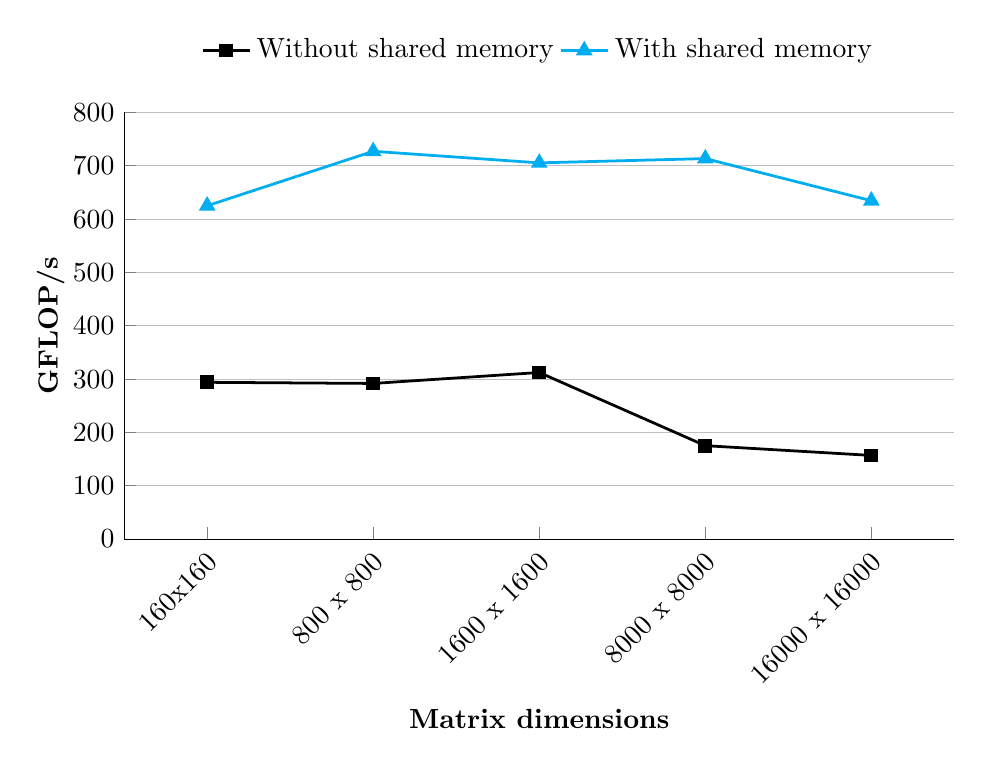
\begin{tikzpicture}
		\begin{axis}
			[
			,width=\textwidth
			,height=7cm
			,axis x line*=bottom
			,axis y line*=left
			,xlabel=\textbf{Matrix dimensions}
			,x label style={at={(axis description cs:0.5,-0.375)},anchor=north,font=\normalsize}
			,ylabel=\textbf{GFLOP/s}
			,y label style={at={(axis description cs:-0.06,.5)},rotate=0,anchor=south,font=\normalsize}
			,xmin=0.5, xmax=5.5
			,ymin=0, ymax=800
			,xtick=data,
			,xtick pos=left
			,ytick={0,100,200,300,400,500,600,700,800}
			,ytick pos=left
			,xticklabels={160x160,800 x 800,1600 x 1600,8000 x 8000,16000 x 16000}
			,x tick label style={rotate=45,anchor=east,yshift=-6pt,align=right,font=\normalsize}
			,y tick label style={font=\normalsize}
			,ymajorgrids
			,scatter/classes={
				shared-mem={mark=square*,blue},
				no-shared-mem={mark=triangle*,black}
			}
			,legend style={at={(0.5,1.2)},anchor=north,font=\normalsize,cells={anchor=east}, legend columns=-1,draw=none}
			]
			\addplot[black,line width=1pt,mark=square*,mark options={mark size=2}] coordinates {
				(1, 293.96) [no-shared-mem]
				(2, 291.84) [no-shared-mem]
				(3, 312.38) [no-shared-mem]
				(4, 175.16) [no-shared-mem]
				(5, 156.85) [no-shared-mem]
			};
			\addplot[cyan,line width=1pt,mark=triangle*] coordinates {
				(1, 625.00) [shared-mem]
				(2, 727.18) [shared-mem]
				(3, 705.41) [shared-mem]
				(4, 713.48) [shared-mem]
				(5, 634.50) [shared-mem]
			};
			\legend{Without shared memory, With shared memory}
		\end{axis}
	\end{tikzpicture}
	\caption{Matrix multiplication results of matrices with varying dimensions; matrices are filled with 1 element. The values - presented in GFlop/s - are averages from 10 loops of the operation.}
	\label{Figure:CUDA-matrix-multiplication-benchmark-results-flops}
\end{figure}

\begin{table}[h!]
	\centering
	\renewcommand{\arraystretch}{1.5}
	\begin{tabular}{ |c|r|r| } 
		\hline
		& \multicolumn{2}{c|}{Results [msec]} \\
		\hline
		\multicolumn{1}{|c}{Matrix dimensions} & \multicolumn{1}{|c}{Without shared memory} & \multicolumn{1}{|c|}{With shared memory} \\
		\hline
		160 x 160 & 0.028 & 0.013 \\
		\hline
		800 x 800 & 3.509 & 1.408 \\
		\hline
		1600 x 1600 & 26.224 & 11.613 \\
		\hline
		8000 x 8000 & 5846.247 & 1435.221 \\
		\hline
		16000 x 16000 & 52226.867 & 12910.967 \\
		\hline
	\end{tabular}
	\caption{Matrix multiplication results of matrices with varying dimensions; matrices are filled with 1 element. The values - presented in milliseconds - are averages from 10 loops of the operation.}
	\label{Table:CUDA-matrix-multiplication-benchmark-results-msec}
\end{table}

As can be seen in Figure~\ref{Figure:CUDA-matrix-multiplication-benchmark-results-flops} and Table~\ref{Table:CUDA-matrix-multiplication-benchmark-results-msec}, the approach that utilizes shared memory achieved between 2-4 times the number of GFLOPs per second and similarly faster execution times compared to the approach that does not use shared memory and instead relies only on global memory. Additionally, the difference seems to be increasing with growing matrix dimensions, however, this statement has not been verified for dimensions greater than 16000 by 16000.



\section{LU Decomposition \TO}
It can be argued that, in recent years, computational systems and software layers allowing developers to use them to their full potential have developed significantly - Nvidia GPUs and CUDA. Subsequently, many novel uses have been found for such powerful computing systems, especially in areas that require results to be available quickly on demand. An example of such an area is solving systems of linear equations. Being one of the fundamental parts of numerical linear algebra, the requirement for their solution arises not only in computer science, but also in physics, engineering, chemistry, etc. \\
While there are many different methods capable of solving a system comprising of more than one linear equation, in this project, Lower-Upper (LU) decomposition will be detailed. \\
In order to show how LU decomposition can be used to solve a simple system of linear equations an example will be presented. 
\par \textbf{First}, it is necessary to introduce the system. For the purpose of the explanation, let the coefficients of the following system of linear equations:

\begin{align}
	a_{11}x_1 + a_{12}x_2 + a_{13}x_{3}&= \,b_1 \nonumber\,, \\ 
	a_{21}x_1 + a_{22}x_2 + a_{23}x_{3}&= \,b_2 \label{Equation:LU-decomposition-system-linear-equations}\,, \\
	a_{31}x_1 + a_{32}x_2 + a_{33}x_{3}&= \,b_3 \nonumber\,,
\end{align}

be re-written into the matrix form

\begin{equation}\label{Equation:LU-decomposition-system-linear-equations-matrix-form-Axb}
	\mathbb{A}\textbf{x} = \textbf{b}\,,
\end{equation}

where

\begin{equation}
	\mathbb{A} = 
	\begin{bmatrix}
		a_{11} & a_{12} & a_{13} \\
		a_{21} & a_{22} & a_{23} \\
		a_{31} & a_{32} & a_{33}
	\end{bmatrix}
	,\quad
	\mathbf{x} = 
	\begin{bmatrix}
		x_{1} \\
		x_{2} \\
		x_{3}
	\end{bmatrix}
	,\quad
	\mathbf{b} = 
	\begin{bmatrix}
		b_{1} \\
		b_{2} \\
		b_{3}
	\end{bmatrix}.
\end{equation}

In order to be able to use LU decomposition, matrix $ \mathbb{A} $ must be a square matrix ($ n\times n $) that is also strongly regular. This requirement can be relaxed to only requiring regularity by properly ordering the rows and columns of the matrix using a permutation matrix $ \mathbb{P} $, however, such a procedure will not be present in this project, and therefore all coefficient matrices are required to be strongly regular.
\par \textbf{Second}, using a \textit{decomposition algorithm} the coefficient matrix $ \mathbb{A} $ is decomposed into the product of a lower triangular matrix $ \mathbb{L} $ and a upper triangular matrix $ \mathbb{U} $:

\begin{equation}
	\mathbb{A} = \mathbb{LU}\,,
\end{equation}

\begin{equation}
	\begin{bmatrix}
		a_{11} & a_{12} & a_{13} \\
		a_{21} & a_{22} & a_{23} \\
		a_{31} & a_{32} & a_{33}
	\end{bmatrix}
	=
	\begin{bmatrix}
		l_{11} & 0      & 0          \\
		l_{21} & l_{22} & 0          \\
		l_{31} & l_{32} & l_{33}
	\end{bmatrix}
	\begin{bmatrix}
		u_{11} & u_{12} & u_{13} \\
		0      & u_{22} & u_{23} \\
		0      & 0      & u_{33}
	\end{bmatrix}.
\end{equation}

Then, substituting Equation~\ref{Equation:LU-decomposition-system-linear-equations-matrix-form-Axb} into Equation~\ref{Equation:LU-decomposition-system-linear-equations-matrix-form-Axb} yields:

\begin{equation}\label{Equation:LU-decomposition-system-linear-equations-matrix-form-LUxb}
	\mathbb{LU}\textbf{x} = \textbf{b}\,.
\end{equation}.

\par \textbf{Third}, the matrix form from Equation~\ref{Equation:LU-decomposition-system-linear-equations-matrix-form-LUxb} is used to obtain the solution to the system of linear equations using forward and backward substitution:

\begin{enumerate}
	\item Solve the equation $ \mathbb{L}\textbf{y} = \textbf{b} $ (where only $ \textbf{y} $ is not known):
	\begin{equation}\label{Equation:LU-decomposition-solving-Lyb}
		\begin{bmatrix}
			l_{11} & 0      & 0          \\
			l_{21} & l_{22} & 0          \\
			l_{31} & l_{32} & l_{33}
		\end{bmatrix}
		\begin{bmatrix}
			y_{1} \\
			y_{2} \\
			y_{3}
		\end{bmatrix}
		=
		\begin{bmatrix}
			b_{1} \\
			b_{2} \\
			b_{3}
		\end{bmatrix}.
	\end{equation}
	\item Solve the equation $ \mathbb{U}\textbf{x} = \textbf{y} $ (where only $ \textbf{x} $ is not known):
	\begin{equation}\label{Equation:LU-decomposition-solving-Uxy}
		\begin{bmatrix}
			u_{11} & u_{12} & u_{13} \\
			0      & u_{22} & u_{23} \\
			0      & 0      & u_{33}
		\end{bmatrix}
		\begin{bmatrix}
			x_{1} \\
			x_{2} \\
			x_{3}
		\end{bmatrix}
		=
		\begin{bmatrix}
			y_{1} \\
			y_{2} \\
			y_{3}
		\end{bmatrix}.
	\end{equation}
\end{enumerate}

It is noteworthy that since the values on the right-hand side (vector $ \textbf{b} $) are only required in step 3 (equations~\ref{Equation:LU-decomposition-solving-Lyb} and \ref{Equation:LU-decomposition-solving-Uxy}), they are not required for the process of decomposition itself. Thus, if there is more than 1 right side in the system of linear equations, matrix $ \mathbb{A} $ needs to be decomposed into matrices $ \mathbb{L} $ and $ \mathbb{U} $ only once; the same principle is valid even if the right side is not known ahead of time. In other words, $ \mathbb{L} $ and $ \mathbb{U} $ can used to solve the system for different right-hand sides without the need for repeated decomposition. Additionally, this concept can be seen as an advantage for LU decomposition compared to Gaussian elimination as the latter requires the right-hand side to obtain the system's upper triangular matrix and subsequently use it for backward substitution. This concept is described, for example, by George Lindfield and John Penny in \emph{Numerical Methods: Linear Equations and Eigensystems} \cite{Lindfield2019}.

In summary, from the steps above, it can argued that the \textit{decomposition algorithm} mentioned in step 2 is one of the key components of the procedure and as such it will be the main topic of this project.

\subsection{Crout method \TO}\label{Subsection:LU-decomposition-crout-method}
This subsection aims to explain in greater detail the decomposition algorithm mentioned above in step 2. There are many different procedures to decompose matrix $ \mathbb{A} $ into matrices $ \mathbb{L} $ and $ \mathbb{U} $ such that $ \mathbb{A} = \mathbb{LU} $. One such procedure, developed by Prescott Durand Croutis, is the \textit{Crout method} - sometimes also referred to as \textit{Crout matrix decomposition} or \textit{Crout factorization} \cite{Press2007}. \\
This method differs from similar procedures in that the resulting $ \mathbb{U} $ matrix is a unit upper triangular matrix, while $ \mathbb{L} $ remains to be a lower triangular matrix. A unit triangular matrix differs from a regular triangular matrix in that its main diagonal is comprised solely of ones. In other words, all elements on the main diagonal of $ \mathbb{U} $ are equal to $ 1 $ ($ u_{11} = u_{22} = u_{33} = 1 $):

\begin{equation}
	\begin{bmatrix}
		1      & u_{12} & u_{13} \\
		0      & 1      & u_{23} \\
		0      & 0      & 1
	\end{bmatrix}.
\end{equation}

\paragraph{Algorithm}
The Crout matrix decomposition algorithm is based on sequentially filling in matrices $ \mathbb{L}_{n\times n} $ and $ \mathbb{U}_{n\times n} $ using elements from matrix $ \mathbb{A}_{n\times n} $. At the core of this filling-in are the following formulas and their conditions for $ l_{ij} $ and $ u_{ij} $:

\begin{align}
	l_{ij} &= a_{ij} - \sum_{k=1}^{j-1}l_{ik}u_{kj} 								   &\quad i \geq j\,, \label{Equation:LU-decomposition-crout-method-lij} \\
	u_{ij} &= \frac{1}{l_{ii}} \left ( a_{ij} - \sum_{k=1}^{i-1}l_{ik}u_{kj} \right ), &\quad i < j\,, \\ \label{Equation:LU-decomposition-crout-method-uij}
	u_{ij} &= 1 																	   &\quad i = j\,, \\
	i,j &\in \widehat{n} \nonumber\,.
\end{align}

Specifically, the algorithm first computes a column $ j $ in $ \mathbb{L} $ and then row $ j $ in $ \mathbb{U} $. This process repeats itself for $ j $ from $ 1 $ to $ n $. The pseudo-code implementing the algorithm can be seen in Listing~\ref{Listing:LU-decomposition-crout-method-pseudocode} and the visualization of the algorithm's advance is shown in Figure~\ref{Figure:LU-decomposition-crout-method-visualisation}.

\begin{lstlisting}[caption={C++ Pseudo-code implementing Crout's matrix decomposition algorithm. It assumes that \code{A[n][n]} is a two-dimensional array that represents the invertible square coefficient matrix $ \mathbb{A} $; \code{L[n][n]} and \code{U[n][n]} are also two-dimensional arrays reprenting matrices $ \mathbb{L} $ and $ \mathbb{U} $ respectively. Furthermore, it is assumed that \code{L} and \code{U} are populated with zeros. Derived from \emph{Crout's LU Factorization} \cite{rqjYYJkSwERYYbSy}, \emph{Numerical recipes: the art of scientific computing} \cite{Press2007} and \emph{Crout matrix decomposition} \cite{TgtpOw7zCHo3ii0m}.},label={Listing:LU-decomposition-crout-method-pseudocode}]
void crout_method(A, L, U) {
	int i, j, k;
	double sum = 0;
	
	// Fill main diagonal of U with 1s
	for (i = 0; i < n; i++) {
		U[i][i] = 1;
	}
	
	// Loop through the main diagonal
	for (j = 0; j < n; j++) {
		
		// Compute column j in L
		for (i = j; i < n; i++) {
			sum = 0;
			for (k = 0; k < j; k++) {
				sum += L[i][k] * U[k][j];	
			}
			L[i][j] = A[i][j] - sum;
		}
		
		// Compute row j in U
		for (i = j; i < n; i++) {
			sum = 0;
			for(k = 0; k < j; k++) {
				sum = sum + L[j][k] * U[k][i];
			}
			if (L[j][j] == 0) {
				printf("det(L) close to 0!\n Can't divide by 0...\n");
				exit(EXIT_FAILURE);
			}
			U[j][i] = (A[j][i] - sum) / L[j][j];
		}
	}
}
\end{lstlisting}

\begin{figure}[h!]
	\centering
	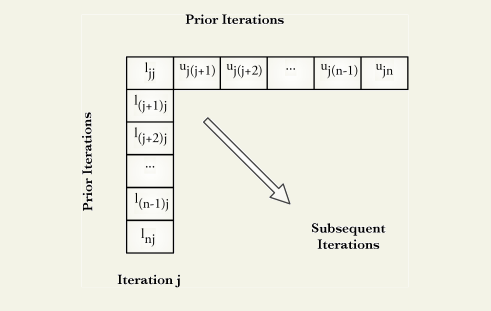
\includegraphics[width=0.8\textwidth, keepaspectratio]{images/ch1/LU_decomposition_crout_method_visualization.png}
	\caption{Sequence of computations of the Crout method. First, column $ j $ in $ \mathbb{L} $ is computed and then row $ j $ of $ \mathbb{U} $. Taken from Vismor's \emph{Crout's LU Factorization} \cite{rqjYYJkSwERYYbSy}.}
	\label{Figure:LU-decomposition-crout-method-visualisation}
\end{figure}

\subsection{Numerical method \TO}\label{Subsection:LU-decomposition-numerical-method}
When solving systems of linear equations there are 2 main groups of methods:

\begin{enumerate}
	\item Direct methods - theoretically, the exact solution will be obtained after a finite amount of steps (e.g. Crout method).
	\item Iterative methods - theoretically, these methods converge to the solution, however, the exact solution is not guaranteed to be found (numerical methods).
\end{enumerate}

The Crout method as described in Subsection~\ref{Subsection:LU-decomposition-crout-method} is a direct method, meaning that it provides an exact solution. Furthermore, it is strictly sequential, meaning that there is seemingly no room for parallelization. \\
However, Hartwig Anzt et al. in their paper \emph{ParILUT - A Parallel Threshold ILU for GPUs} \cite{Anzt2019} describe different approaches to generating incomplete factorizations. An example of such a group of approaches is referred to as \textit{ParILU algorithms} which are distinct in the fact that they abandon the methodology akin to Gaussian elimination. Rather, these methods use "\textit{fixed-point iterations to approximate the incomplete factors on a pre-defined sparsity pattern}" - iterative methods. The authors in the paper explain method belonging to this group as algorithms that do not take every non-zero into account. \\
However, for the purpose of this paper, it was decided to derail from this principle - exclude any sparsity pattern conditions - and focus purely on the iterative aspect of the methodology. In other words, use the fixed-point iterating algorithm that - according to the authors - converges to a sufficiently approximate solution of $ \mathbb{A} = \mathbb{LU} $ without taking into account sparsity patterns. \\
Specifically, the algorithm is as follows:

\begin{enumerate}
	\item Provide an initial guess (estimate) of matrices $ \mathbb{L}^0 $ and $ \mathbb{U}^0 $. For example, using $ \mathbb{A} $:
		\begin{align}
			l_{ij}^{0} &= a_{ij} \quad &i < j \nonumber\,, \\
			u_{ij}^{0} &= a_{ij} \quad &i > j \nonumber\,, \\
			u_{ij}^{0} &= 1 \quad      &i = j \nonumber\,.
		\end{align}
	\item Using the formulas in Equations~\ref{Equation:LU-decomposition-crout-method-lij} and \ref{Equation:LU-decomposition-crout-method-lij} calculate the next iteration of $ \mathbb{L}^{t} $ and $ \mathbb{U}^{t} $ (where $ t \in \widehat{\mathbb{N}}_0 $ denotes the iteration): $ \mathbb{L}^{t+1} $ and $ \mathbb{U}^{t+1} $
		\begin{align}
			l_{ij}^{t+1} &= a_{ij} - \sum_{k=1}^{j-1}l_{ik}^{t}u_{kj}^{t} 								   &\quad i \geq j \nonumber\,, \\
			u_{ij}^{t+1} &= \frac{1}{l_{ii}^{t}} \left ( a_{ij} - \sum_{k=1}^{i-1}l_{ik}^{t}u_{kj}^{t} \right ) &\quad i < j \\ \nonumber\,.
		\end{align}
	\item If either $ \left | \mathbb{L}^{t+1} - \mathbb{L}^{t} \right | $ or $ \left | \mathbb{U}^{t+1} - \mathbb{U}^{t} \right | $ is greater than some tolerance, e.g. $ 0.001 $, then go back to step 2.
	\item If both differences are smaller than the tolerance, then the algorithm has iteratively converged to an approximate solution of $ \mathbb{A} = \mathbb{LU} $.
\end{enumerate}

On one hand, the number of iterations it takes the algorithm to converge to a solution is not possible to accurately predict and therefore could lead to poor performance if performed sequentially. On the other hand, since $ \mathbb{L}^{t+1} $ and $ \mathbb{U}^{t+1} $ are calculated independently, the operation can be run in parallel. \\
Another noteworthy, but unverified, aspect of this method's convergent nature is related to rounding errors. Specifically, since Crout's method is direct, it can be theorized that rounding errors may result in it providing less accurate results compared to its numerical modification. This thought stems from the fact that the numerical method converges and thus - under specific convergence rules - may arrive at a more accurate solution. However, this is purely a hypothesis and remains to be verified. \\
Joining together the highly parallel nature of CUDA-enabled Nvidia GPUs and such a heavily parallelizable algorithm is the main focus of this project and will be detailed further in the following chapters.
